\chapter{Морская практика в дальнем плавании}

Яхтенный капитан должен твёрдо знать, что море ошибок не прощает, обязан постоянно совершенствовать своё мастерство, с каждым плаванием обогащать личный опыт моряка\-/спортсмена. Руководствуясь правилами <<хорошей морской практики>>, яхтенному капитану следует не только тщательно и всесторонне готовить своё судно и экипаж к предстоящему плаванию, но и во всех сомнительных случаях, будь то метеоусловия или навигационная обстановка, всегда считать себя <<ближе к опасности>>. Такой разумный и учитывающий все обстоятельства подход обеспечит безопасность плавания.

\section{Управление крейсерско\-/гоночными яхтами в штормовую погоду}

\begin{figure*}[htb]
  \centering{}
  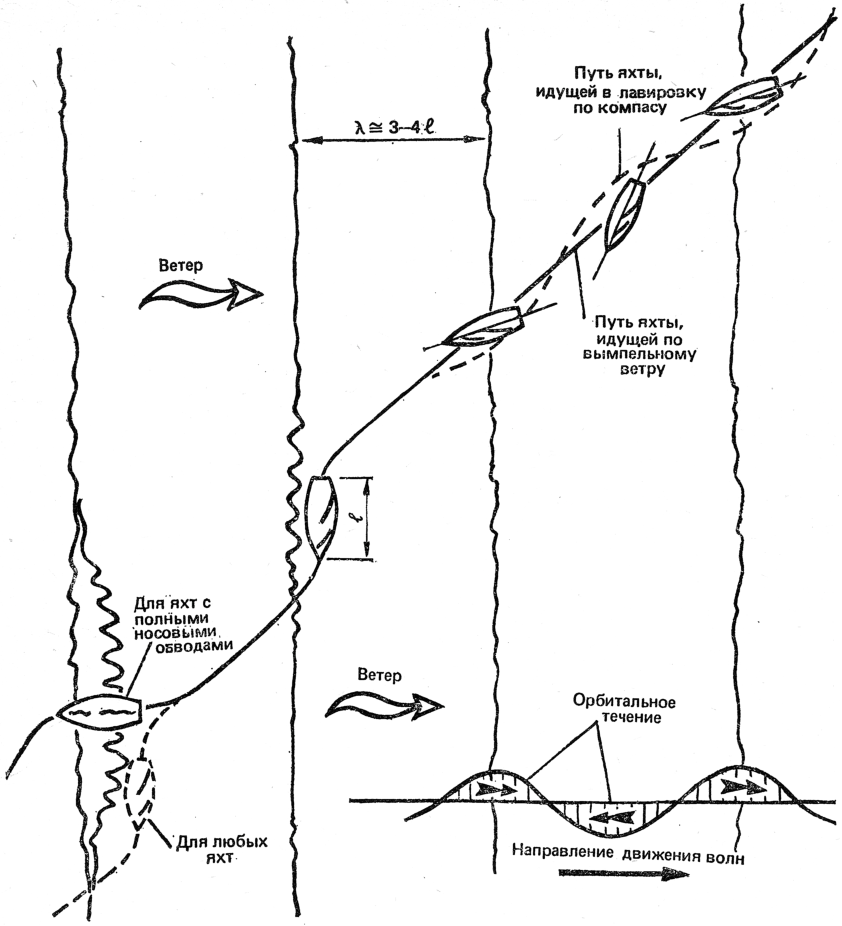
\includegraphics[scale=1.3]{0128P}
  \caption{Плавание против встречного волнения}
  \label{fig:128}
\end{figure*}

Капитан яхты, застигнутый в море штормом, прежде всего должен решить вопрос о целесообразности продолжения плавания. Если район плавания изобилует навигационными опасностями, то необходимо укрыться в ближайшем порту\-/убежище, гавани на закрытом рейде, особенно при плохой видимости. Но если опасностей по курсу нет, плавание лучше продолжать, так как риск захода в порт больше, особенно если он незнаком.

В шторм курс яхты следует прокладывать дальше от берега, чтобы не попасть на прибойную волну и иметь под ветром место для вынужденного дрейфа в случае аварии или при смене парусов. Во время сильного шторма не следует без особой необходимости делать повороты как через фордевинд, так и оверштаг. При неумелых или неудачных поворотах в первом случае можно порвать парус, сломать гик и мачту, а во втором \--- порвать задние шкаторины парусов. Если же есть необходимость в повороте через фордевинд, то следует разогнать яхту на курсе бакштаг на подветренном склоне волны, быстро добрать гика\-/шкот в тугую и повернуть на вершине пологой волны, выждав момент ослабления ветра. Во время поворота не рекомендуется отдавать наветренный бакштаг, пока не будет заложен подветренный. Иначе его не удастся <<набить>> после поворота.

Поворот оверштаг в шторм нужно делать очень быстро на вершине пологой волны, не имеющей гребня. Перед поворотом и после него необходимо немного валиться с целью быстрее набрать ход. В свежий ветер при поворотах оверштаг гика-шкотом не работают.

Если шторм застаёт яхту в гонке, то достаточно опытный экипаж может допустить форсирование парусами. На курсе галфвинд необходимо добрать оттяжку гика, а при особо сильных порывах немного потравить гика\-/шкот, чтобы ослабить нагрузку на руль. На курсах бакштаг и фордевинд грот должен быть плоским, поэтому втугую набивают оттяжку гика. На курсе бейдевинд следует брать рифы и заменять передние паруса, не допуская крена яхты более более 30\gr.
 
\textbf{Техника плавания на волне.} Для яхт не так опасен ветер, как высокие и крутые волны, которые могут опрокинуть её вверх килем, сорвать люки, сломать мачты, разбить корпус. Поэтому для управления яхтой на волне нужна специальная техника.

При лавировке на большой волне, чтобы не терять ход, надо идти несколько полнее, потравив немного шкоты. Когда длина волны становится равной примерно длине корпуса, яхту начинает бить о волну, сбивать ход и <<вытряхивать>> ветер из парусов. Чтобы изменить период продольной качки, приходится уваливаться. При длине волны, равной двум корпусам судна, продольная качка становится более спокойной, но затрудняется управление яхтой. Орбитальным течением волн её то приводит, то уваливает.

При длине волны, равной трём\-/четырём корпусам, можно идти быстрее и круче, если править не по компасу, по вымпельному ветру так, чтобы курсовой угол вымпельного ветра был постоянным. В ложбине между волнами рулевой должен немного изменять курс под ветер, а на гребнях волн \--- на ветер (рис.~\ris{128}). При управлении по вымпельному ветру фактический путь яхты ближе к прямому, чем если бы она шла по компасу. Для того чтобы избежать замедления хода, сильного удара и заливания яхты на гребнях особо крупных волн, следует перед ними уваливаться до угла 50\otdo 60\gr к направлению бега волны, а затем снова приводиться на постоянный курс. Иногда крутые волны лучше встречать носом, почти перпендикулярно к гребню (в частности, на яхтах с полными носовыми обводами), а после его прохождения уваливаться.

На полных курсах волны обгоняют тяжёлые яхты. Чтобы использовать энергию попутных волн для ускорения хода, следует меньше времени идти на наветренной стороне гребня и больше на подветренной. Для этого сразу после прохождения гребня нужно приводиться до бакштага и разгонять яхту, а перед крутым склоном набегающей волны уваливаться на фордевинд и идти сколько можно в режиме сёрфинга (рис.~\ris{129}).

При плавании в шторм особо опасны банки и отличительные глубины в море и надо обходить их стороной. На глубинах менее половины длины волны увеличивается высота волны и образуются опасные буруны.

\begin{figure*}[htb]
  \centering{}
  \includegraphics[scale=1.3]{0129P}
  \caption{Плавание с попутным волнением}
  \label{fig:129}
\end{figure*}

{\small 28 сентября 1975 г. двухмачтовая яхта <<Кедровник>> (типа <<Опал>>) в районе острова Гельголанд в Северном море попала в зону набирающего силу урагана. В 4~ч 47~мин на яхту обрушилось несколько необычно высоких волн, которые перевернули её, сломав обе мачты, выбив иллюминаторы и залив наполовину. Экипаж не пострадал, в момент аварии на палубе был один рулевой, привязанный страховочным поясом. При перевороте с палубы сорвало спасательный плот, который раскрылся и был унесён ветром. Потеря плота подхлестнула энергию яхтсменов. Они подняли на борт сломанный рангоут, откачали воду, поставили вместо мачты спинакер\-/гик и под апселем ушли под прикрытые острова Гельголанд. Как считают, яхта попала в район с резкой сменой глубин, где в шторм образовался бурун, опрокинувший яхту.}

\textbf{Плавание под штормовыми парусами.} В зависимости от силы ветра, курса, мореходности и водоизмещения яхты, квалификации экипажа и условий плавания в шторм на гроте берут рифы и меняют большие передние паруса на меньшие. Техника взятия рифов традиционным способом, с помощью сезней, в настоящее время настолько усовершенствовалась, что на всю операцию тратится не более 30~сек. На вертлюге гика крепится гак или штырь с головкой, на которую, осадив грот, надевается передний люверс нужного ряда рифов (см. рис.~\ris{45}). Риф\-/шкентель, заранее заведённый в кренгельс на задней шкаторины, выбирается втугую талями или лебёдкой и закладывается на гребёнке на гике. При этом, разумеется, работают ещё с грота\-/фалом, топенантом и гика шкотом. Свободную мякоть паруса не очень туго скатывают и шнуруют через люверсы, пробные на гроте примерно через 75\otdo 90~см. 

\begin{figure}[htb]
  \centering{}
  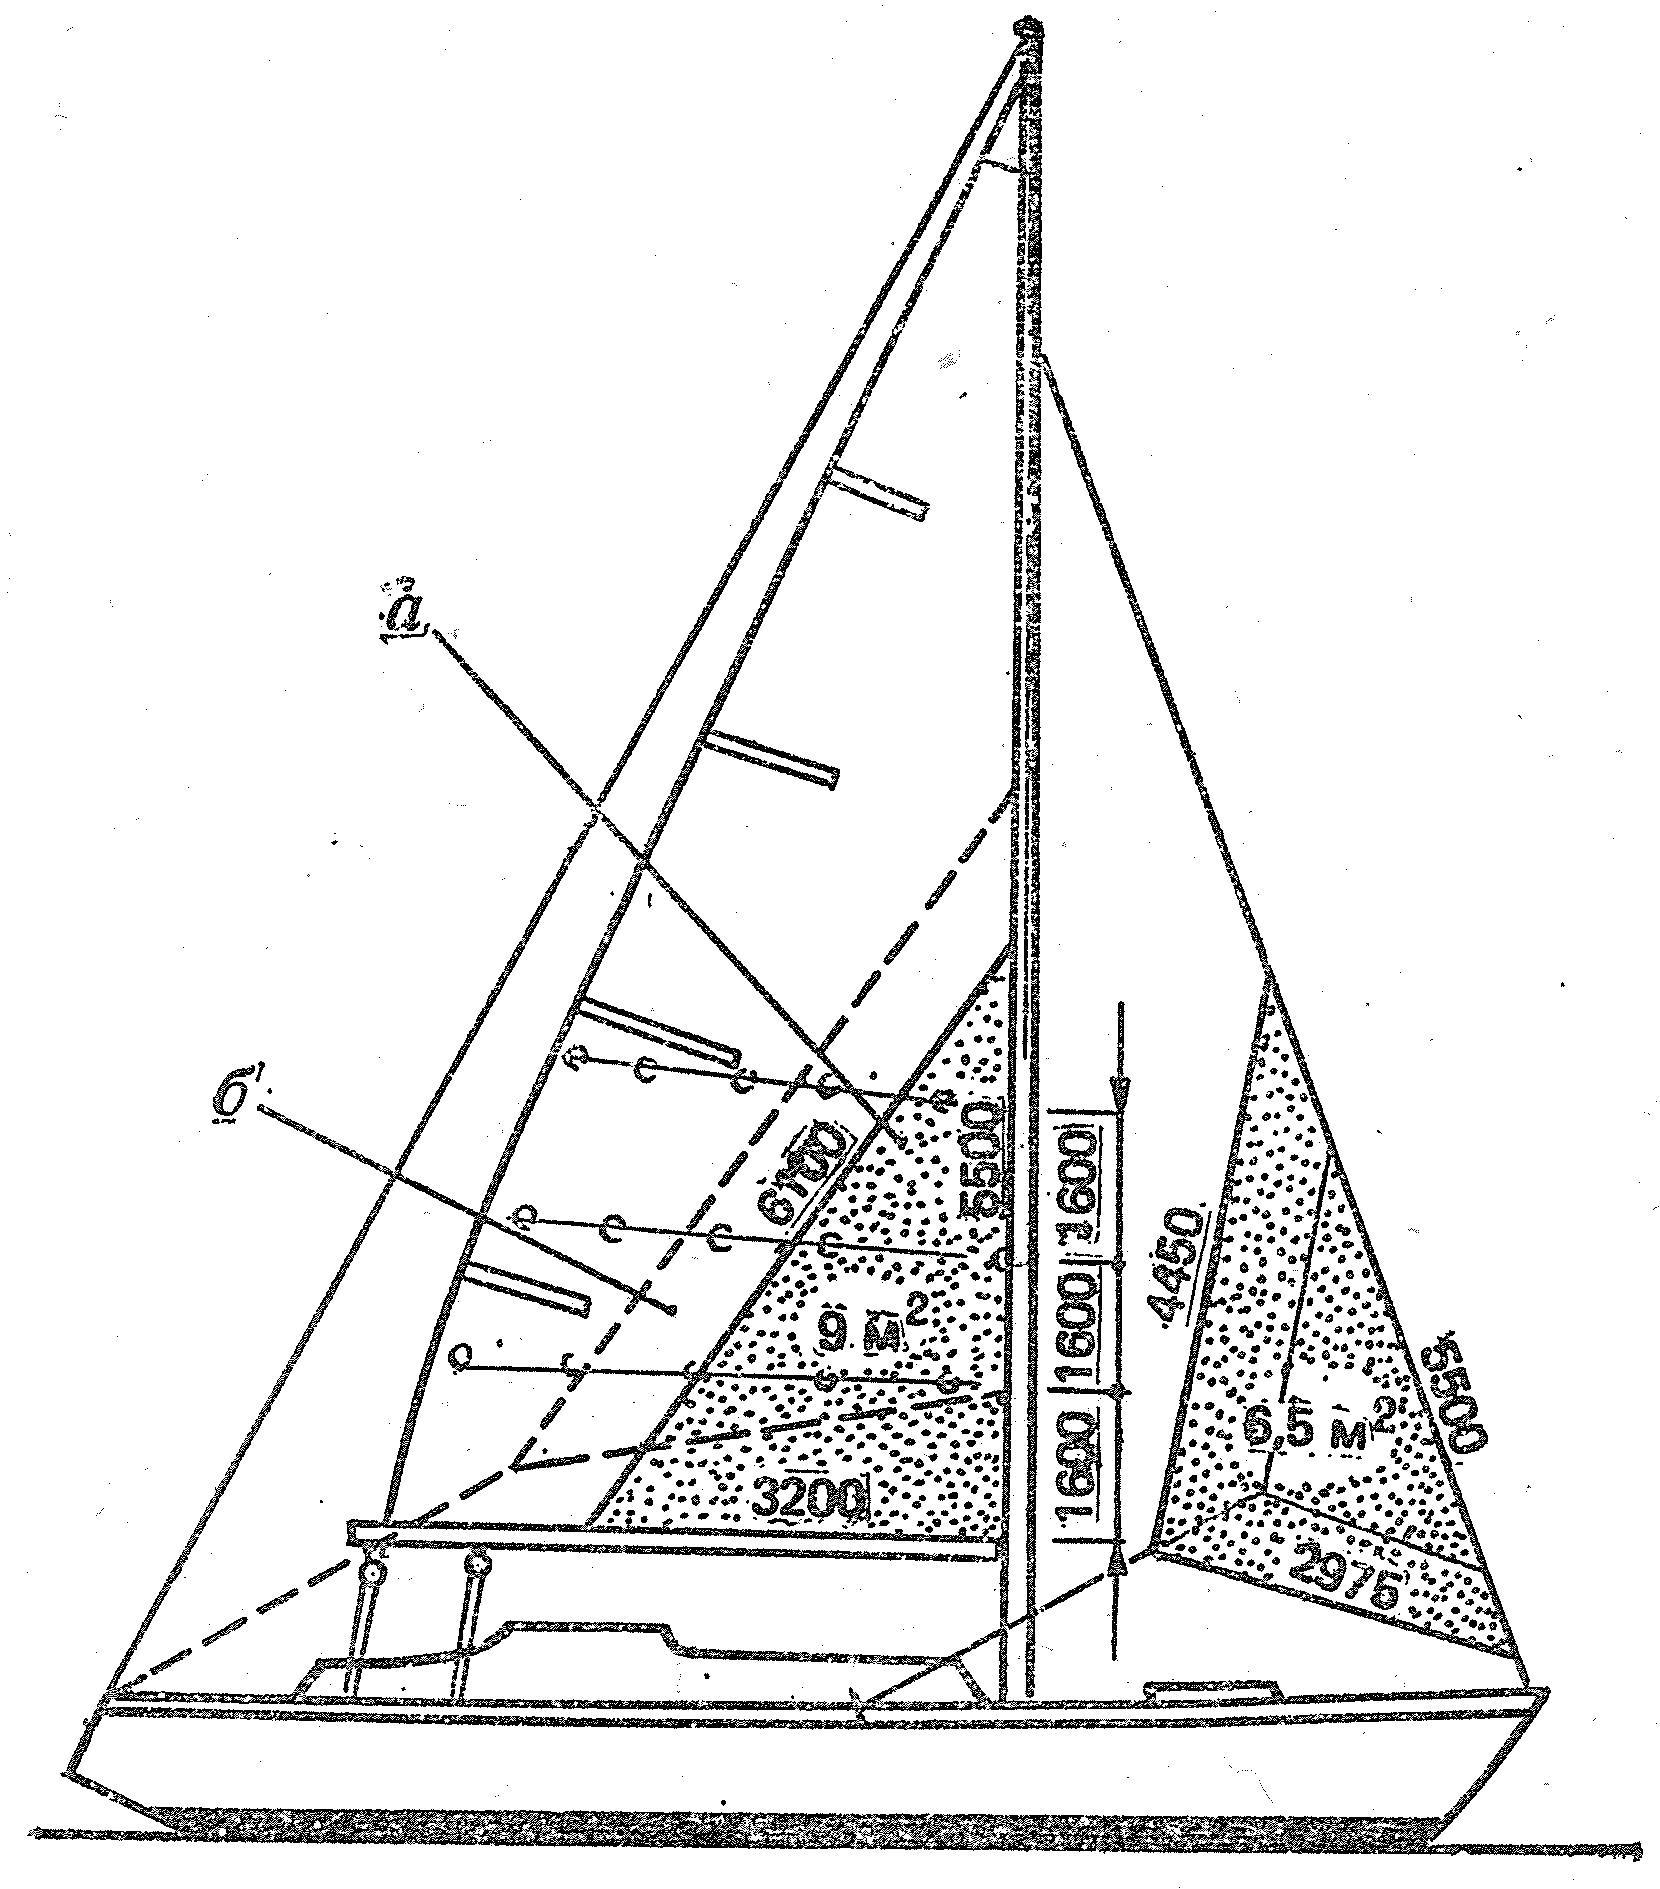
\includegraphics[scale=1.2]{0130P}
  \caption{Штормовые паруса на яхте класса Л-6}
  \label{fig:130}
  \small
  \centering{}
  \textbf{а} \--- трисель с высоким шкотовым углом; \textbf{б} \--- трисель с низким шкотовым углом
\end{figure}

\begin{figure*}[htb]
  \centering{}
  \includegraphics[scale=1.3]{0131P}
  \caption{Различные способы постановки яхты в дрейф}
  \label{fig:131}
\end{figure*}

Этот способ взятия рифов применим только для прочных дакроновых парусов. Схема примерного расположения рифов на гроте яхты типа Л-6 показана на рис.~\ris{130}. Согласно принятой международной практике, последний ряд рифов на гроте должен уменьшать площадь паруса на 50\,\%. 

При ветре силой 10 баллов и более на яхтах ставят трисели и штормовые стаксели. Для малых яхт и на лавировке этот момент может наступить раньше, чем для больших яхт и на полных курсах. 

Трисели могут различаться по форме (с низким или высоким шкотовым углом) и по способу крепления шкотового угла (на гике или на корме). Трисели с низким шкотовым углом и креплением шкотов на корме лучше использовать при сильном волнении, когда яхта часто оказывается между гребнями высоких волн. Правда, такой парус плохо стоит на курсе фордевинд. Трисели с высоким углом и креплением шкотового угла на гике позволяют идти круче к ветру на сравнительно гладкой воде (см. рис.~\ris{128}) и лучше стоят на полных курсах. В этом случае во избежание поломки гика точка крепления шкотового угла должна совпадать с точкой крепления гика\-/шкота.

Лежание в дрейфе и на плавучем якоре. Когда с усилением ветра идти становится тяжело, а шторм не попутный и под ветром есть достаточно места, то ложатся в дрейф под парусами либо встают на плавучий якорь. Если же под ветром опасно, можно удерживаться на месте, лавируя под триселем.

Наиболее устойчиво лежат в дрейфе одномачтовые и двухмачтовые яхты под двумя парусами: выбранными втугую триселем и штормовым стакселем, вынесенным на ветер (рис.~\ris{131}, \textit{а}, \textit{б}). Руль крепят либо в \textit{ДП}, либо немного перекладывают на ветер, в зависимости от свойств яхты. В этом положении яхта стоит под углом 50\otdo 60\gr к ветру, дрейфуя под ветер со скоростью 1,5\otdo 2~узла. 

На иолах и кэчах иногда дрейфуют под глухо зарифленной и выбранной в \textit{ДП} бизанью и штормовым стакселем, вынесенным на ветер, но в этом случае дрейф менее устойчив (рис.~\ris{131}, \textit{в}). Можно дрейфовать под одним штормовым стакселем. Для этого стаксель\-/шкот выбирают втугую с полветра, а руль кладут на ветер и крепят. В этом случае яхта будет дрейфовать по принципу <<падающего листа>>, то набирая ход и приводясь, то теряя его и уваливаясь (рис.~\ris{131}, \textit{г}). Суммарная скорость дрейфа тогда составит 3~уз и более. Яхта может дрейфовать и под одним рангоутом с рулём, положенным на борт (рис.~\ris{131}, \textit{г}), однако скорость дрейфа в таком случае окажется значительно больше 3~узлов.

По схемам, показанным на рис.~\ris{131} (\textit{а}, \textit{б}, \textit{е}, \textit{ж}), можно ложиться в дрейф не только в шторм, но и при нормальной погоде под полными парусами (гротом и генуей), когда хотят быстро остановить яхту, не становясь на якорь, и есть место для дрейфа. На рис.~\ris{131}, \textit{е} и \textit{ж} (шлюп и кэт) грот растравлен до вант.

Если из-за высоких гребней волн, опрокидывающихся на яхту, дрейфовать становится небезопасно, то отдают с носа плавучий якорь, который разворачивает судно носом против ветра и волны. Скорость дрейфа на плавучем якоре 2\otdo 3~уз (в зависимости от условий). Чем сильнее волнение, тем на большую длину следует вытравливать якорный канат (дректов). При уборке якоря выбирают предназначенный для этой цели вытяжной трос, который во время отстаивания на плавучем якоре вытравливают на большую длину, чем якорный канат. Следует иметь в виду, что орбитальным движением воды вытяжной трос может закрутиться вокруг якорного каната, тогда невозможно будет его использовать. 

Убегание от шторма \--- это уход от ветра и волны полным курсом с наибольшей скоростью. Если сила ветра позволяет, то это делают под триселем и штормовым стакселем. В таких условиях трисель шкоты обязательно крепить на корме яхты, а не на гике, так как при большом крене гик обязательно заденет за волну и сломается. Чтобы избежать случайного разворота яхты лагом к волне при разыскивании, с кормы полезно вытравить несколько тросов длиной около 40\otdo 50~м каждый или небольшой плавучий якорь. Если шторм переходит в ураган, то оставляют один штормовой стаксель или уходят под одним рангоутом. При скорости ветра 33~м/с, например, удельное давление ветра достигает 90\kgmsq. 

При убегании от шторма на фордевинд ни в коем случае нельзя допускать непроизвольных перебрасываний стакселя с борта на борт, иначе от стакселя отрываются карабины, рвутся фалы и шкоты, разбалтываются крепления штага. Чтобы этого избежать, достаточно немного изменить курс с фордевинда на полный бакштаг.

Штормовать в море или зайти в укрытие - решает капитан яхты, исходя из следующих предпосылок: 
\begin{itemize}
\item общий маршрут, место судна и его курс, близость берега, наличие укрытий и характер подходов к ним, глубины, фактический ветер и волнение, прогноз погоды, местные признаки; 
\item состояние корпуса, рангоута, такелажа, парусов и снабжения; 
\item квалификация и физическое состояние команды. 
\end{itemize}

Большинство аварий происходит при заходе яхт в гавань или выходе из них во время шторма, так как помимо прибойной волны образуется береговое течение, которое сильно сносит яхту с курса и может сделать её неуправляемой. Два примера иллюстрируют это.

{\small Осенью 1975 г. яхта "Комар" в 11-балльный шторм входила в польский порт Дармово на южном побережье Балтийского моря. У входа в порт были высокие, крутые волны. Яхта попыталась уйти обратно в море, но прибойной волной её перевернуло, сломало мачту и выбросило на волнолом.

В 1976 г. яхта "Центаур", возвращаясь из Варнемюнде в Гдыню, попала в 8-балльный шторм. Решили укрыться в порту Владыслово, куда входили под парусами на фордевинд. Яхта сильно рыскала на курсе и раскачивалась с борта на борт. Прибойная волна и прибрежное течение бросили судно на звездообразные блоки мола.}

Общая рекомендация по управлению небольшими парусниками в шторм такова: если курс судна проходит вблизи берега, а надвигающийся шторм ожидается с моря, парусным судам рекомендуется заблаговременно изменить курс с расчётом отойти от берега в сторону моря. Это необходимо, чтобы вовремя уйти с мелководья, от прибойной волны, и иметь запас чистой воды с подветра для маневрирования на случай аварийных ситуаций и т.\=,п. 

В шторм видимость, как правило, ухудшается и снижается точность обсерваций. Поэтому наименьшее расстояние, на которое судно может приблизиться к берегу в шторм, это сумма допустимой по навигационным условиям дистанции сближения с берегом и наибольшей возможной ошибки счисления в сторону опасности. 

Только хорошо изученные и известные пункты с хорошими подходами могут быть надёжными убежищами в шторм. Для того чтобы изучать такие пункты, в учебных плаваниях и при хорошей погоде нужно как можно чаще заходить в них. Однако в учебные плавания с неопытными экипажами не следует выходить в море при падающем давлении и других признаках надвигающегося шторма, характерных для данного района. Маршрут таких плаваний следует планировать вблизи укрытий, до которых можно дойти за 4\otdo 6~часов; не следует выходить на ночь, если по прогнозу ожидается туман, а маршрут проходит вблизи навигационных опасностей. 

При организации и проведении учебных плаваний малых яхт с малоопытными экипажами надо иметь в виду, что после дня лавировки в шторм обычно необходимы два-три дня стоянки для ремонта, просушки парусов, имущества и отдыха команды. 

Техника безопасности в штормовых условиях. Капитан яхты лично ответствен за инструктаж экипажа яхты по технике безопасности работ, выполняемых на палубе и на мачте, при маневрах с парусами, по авральным и аварийным расписаниям, тревоге <<Человек за бортом!>> и т.\=,д., а также за периодическое проведение учебных тревог. 

Наиболее сложные и потенциально опасные работы (оказание помощи терпящему бедствие судну, работы на мачте, завоз якоря) должны выполнять самые квалифицированные матросы под личным контролем капитана яхты или вахтенного начальника.

При первых признаках приближающегося шторма необходимо задраить люки, вентиляционные горловины, иллюминаторы, приготовить внутри яхты принадлежности для взятия рифов, трисель и штормовой стаксель, а если надо, то взять заранее рифы и сменить стаксель на меньший. Все яхтсмены, выходящие на палубу во время шторма, должны быть одеты в непромокаемые костюмы, спасательные жилеты и страховочные пояса, причём при работе на палубе они должны быть пристёгнуты карабином к специальным рамам, реслингам или страховочным леерам. Страховочный леер протягивают от носа до кормы с обоих бортов вдоль фальшборта или комингса рубки. Он удобен тем, что, заложив за него карабин, яхтсмен может свободно передвигаться по всей длине яхты. Страховочный леер заводят со слабиной и поддерживают в натянутом состоянии с помощью резинового стропа, так как туго натянутый леер легко может порваться даже при небольшой нагрузке.

Хождение по подветренной стороне палубы во время шторма должно быть запрещено за исключением случаев, связанных с выполнением конкретных работ. При взятии рифов, перед работами на гике проверяют, хорошо ли заложен топенант и гика\-/шкот. При сильном ветре для взятия рифов грот убирают на палубу, после чего ставят снова.

Если при смене стакселей бак сильно заливает водой, а места кругом достаточно, \--- необходимо увалиться. 

В дополнение к правилам и нормам обеспечения безопасности морская практика требует соблюдения следующих условий:
\begin{itemize}
\item на морских яхтах не должны применяться задвижные щитки люков, выпадающие при переворачивании яхты; 
\item якоря, аккумуляторные батареи, огнетушители и другие тяжёлые предметы должны быть закреплены во избежание смещения с места или падения при перевороте яхты; 
\item на дверцах и щитках люков не должно быть жалюзи; должны быть аварийные закрытия всех отверстий в палубе и рубке; 
\item на яхте должен иметься плавучий якорь; 
\item мачта в пяртнерсе должна быть расклинена. 
\end{itemize}

Практика показывает, что даже отсутствие таких прозаических деталей в оборудовании яхты, как мойка на камбузе и гальюн, может привести к падению людей за борт.

\section{Особые случаи в плавании}

\textbf{Плавание в узкостях.} К узкостям относятся проливы, шхеры, фарватеры и каналы, расположенные в непосредственной близости от навигационных опасностей.

В особо сложных районах следует уменьшить скорость яхты до пределов, обеспечивающих только выполнение необходимых маневров.

При плавании в узкостях фалы должны быть разобраны, якорь готов к отдаче, команда яхты должна находиться в готовности на верхней палубе. Следует избегать ситуаций, ведущих прямо к аварии: когда яхта идёт курсом крутой бейдевинд впритирку к наветренной бровке фарватера; когда у идущей курсом круто бейдевинд яхты с наветра в непосредственной близости оказывается судно с механическим двигателем, а с подветра, тоже вблизи, бровка фарватера.

В первом случае при внезапном заходе ветра яхта ложится в дрейф и садится на камни, во втором \--- заход ветра ведёт к столкновению с судном либо к посадке на мель.

\textbf{Подход к незнакомому месту стоянки.} При подходе к незнакомому пункту с нехарактерными приметами, следует сначала выйти на ближайший к нему приметный ориентир (маяк, мыс, остров, гора), определить место яхты и затем по прокладке идти в нужное место. При этом необходимо следить за показаниями эхолота и не заходить за безопасную изобату от полутора до двух осадок яхты.

При подходе к неизвестному берегу или незнакомому месту с подводными опасностями, например к отдельным камням, следует вытравить якорь на цепи на гарантированную глубину и уменьшить ход. При плавании на мелководье в незнакомом месте нужно уменьшить крен, убрав лишние паруса или взяв рифы, так как яхту, севшую на мель на ровном киле, снять с неё значительно проще и быстрее. Если судно лавирует в районе с глубинами меньше 1,5 его осадки, то повороты оверштаг делают резко, чтобы в случае задевания фальшкилем за грунт яхта не остановилась, а по инерции закончила поворот и легла на другой галс.

\textbf{Плавание в тумане.} При первых признаках ухудшения видимости необходимо срочно уточнить своё место. В тумане возможны два вида плавания: вдоль береговой черты или в открытом море.

Берег \--- лучший ориентир. Если позволяет глубина и плотность тумана, то можно идти вдоль берега. Когда туман станет густым, следует стать на якорь (желательно в закрытой бухте или гавани) либо уйти в море. Если яхта идёт в тумане вдоль берега, не видя его, необходимо так располагать свой курс, чтобы путь (\PU) уводил её от берега. В тумане желательно уйти из района оживлённого судоходства. В случае сомнения в своём счислимом месте нужно немедленно встать на якорь, лечь в дрейф или уйти в сторону заведомо чистой воды. 

В тумане яхта, согласно требованиям МППСС-72, должна идти безопасной скоростью, подавать туманные сигналы, поднять пассивный радиолокационный отражатель (если его не несут постоянно) и вести наблюдение за чужими сигналами. Безопасная скорость для яхты в тумане \--- нормальный ход, под которым она имеет наибольшую маневренность и управляемость. 

Следует иметь в виду, что звук яхтенного туманного горна не слышен на большом судне из-за шума машин. Поэтому, если пеленг на сигналы приближающегося судна не меняется, полезно обратить его внимание звуковой ракетой и если на яхте есть двигатель \--- запустить его. Когда в тумане начнёт вырастать силуэт приближающегося судна, не рекомендуется делать никакого маневра до тех пор, пока не выяснится его курс, после чего следует действовать быстро и хладнокровно, отворачивая в сторону от курса этого судна.

\section{Посадка на мель и техника снятия с мели в различных условиях}

Посадка на мель может случиться по вине экипажа либо быть результатом стечения непредвиденных обстоятельств. Работы по снятию яхты с мели должны вестись грамотно и энергично, не дожидаясь посторонней мощи. При первом же ударе фальшкилем о грунт необходимо действо таким образом. Если известно, с какой стороны мель, то следует быстро сделать поворот или изменить курс в сторону глубокой воды.

Если расположение мели неизвестно, то с курсов бейдевинд и галфвинд необходимо сразу делать поворот оверштаг и разворачиваться на обратный курс, с полных курсов (фордевинд и бакштаг) выбирать шкоты и приводиться до бейдевинда, а дальше действовать по обстоятельствам. 

Когда сняться с мели с первой попытки ни с помощью парусов, ни с помощью футштоков или двигателя не удаётся, необходимо растравить шкоты или даже убрать лишние паруса, чтобы яхту не тащило дальше на мель, и измерить глубину вокруг яхты. После промера глубин завозят якорь: для разворота \--- по траверзу с бака, а для стягивания \--- прямо по носу или с кормы. Для облегчения разворота и снятия с мели яхту закренивают, посылая людей к подветренным вантам, на гик или подвешивая под гиком тузик, залитый водой. В дополнение к штатному топенанту для усиления заводят на нок гика какие-нибудь свободные фалы. Нельзя переносить гик с борта на борт, если на нем находятся люди. Куда кренить яхту \--- зависит от многих обстоятельств. Обычно на первом этаже не, когда судно только разворачивают, её кренят под ветер. На втором этапе, когда яхту стягивают с мели, крен создают в сторону глубокой воды, что препятствует дальнейшему дрейфу на мель.

Если судно снять с мели не удаётся, а ветер и волнение сильные, надо позаботиться, чтобы судно не разбил волной о грунт. В зависимости от конкретных обстоятельств, яхту можно частично залить водой, чтобы она плотнее села на грунт, либо полностью, если она оказалась на мелком месте, чтобы, когда погода успокоится, можно было снять её с мели с помощью буксирного судна, предварительно откачав воду.

Существуют два способа снятия с мели с помощью буксира.
\begin{description}
\item[Первый способ] \--- буксирный конец закладывают за основание мачты у палубы. Буксирное судно сперва разворачивает, а затем стягивает уже закреплённую силами команды яхту. При этом надо следить, чтобы буксирный трос не перерезало стоячим такелажем яхты и чтобы он не мог соскользнуть вверх по мачте к краспицам.
\item[Второй способ] \--- буксирный конец закладывают за мачту наверху в районе крепления штагов и бакштагов. Этот способ применяют, когда буксирное судно маломощное или когда на большой яхте малочисленный экипаж не может закрепить её своими силами. Тогда буксирное судно одновременно кренит яхту и стягивает с мели в направлении, перпендикулярном диаметральной плоскости. Это очень действенный метод, но следует иметь в виду, что при стягивании яхта может получить ход вперёд и сесть на мель ещё основательнее.
\end{description}

\section{Якорная стоянка}

Якорная стоянка может быть на открытом рейде или в защищённой гавани. Вид стоянки выбирают в зависимости от её цели и продолжительности, состояния судна и погодных условий. Учитывают также, в какой степени якорная стоянка закрыта от ветра и волнения, насколько безопасен подход к ней, какие глубины и какой грунт, есть ли приливы и течения в данном месте и есть ли возможность сняться с якоря и уйти в море при внезапной перемене направления ветра.

Лучшие грунты для стоянки на якоре \--- глина, суглинок, ил с песком и густой ил. Хуже держат якорь песок, ракушка и мелкий камень. Совсем не держат плита и жидкий ил. Дно в районе якорной стоянки должно быть чистым, ровным или почти ровным. На открытых рейдах следует остерегаться большого волнения с моря. При выборе места длительной стоянки на якоре необходимо учитывать возможность разворачивания яхты под действием ветра и течений, вытравливания якорной цепи на полную длину, а также дрейфа яхты и наличия необходимого пространства для маневрирования в случае неудачной съёмки с якоря.

\begin{figure*}[htb]
  \centering{}
  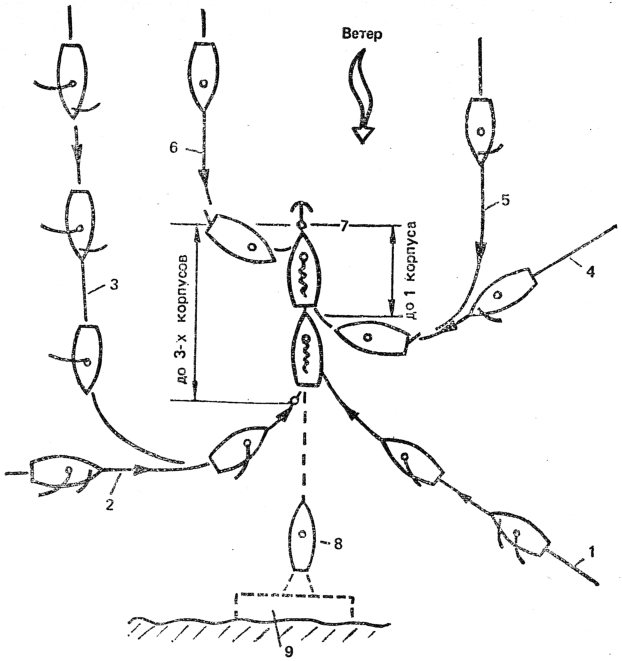
\includegraphics[scale=1.3]{0132P}
  \caption{Схемы подхода к якорной стоянке}
  \label{fig:132}
  \small
  \centering{}
  \textit{1}, \textit{2} и \textit{3} \--- под гротом и стакселем с разных курсов; \textit{4}, \textit{5} \-- под стакселем в свежий ветер на фордевинд и в бакштаг; \textit{6} \--- под рангоутом на фордевинд в шторм; \textit{7} \--- место отдачи якоря; \textit{8} \--- место стоянки на якоря; \textit{9} \--- вариант подхода к пирсу 
\end{figure*}

\textbf{Техника постановки на якорь.} Из множества способов и вариантов постановки яхты на якорь мы рассмотрим несколько основных, наиболее часто применяемых в яхтенной практике (рис.~\ris{132}). 

По команде <<Приготовиться к постановке на якорь!>> отдают с якоря найтовы, вооружают его (если он адмиралтейский) и выкатывают на палубу не менее трёх глубин якорного каната. Одновременно разбирают бухты фалов. 

К месту якорной стоянки подходят кратчайшим путём, по возможности носом против ветра и течения, а при их противоположном действии \--- против того, что действует сильнее. Если нет уверенности, что дно в данном месте чистое (а это при использовании якорей типа <<Данфорта>> всегда желательно), к тренту якоря крепят буйреп с томбуем. Длина буйрепа берётся немного больше глубины. Когда место якорной стоянки находится в закрытой гавани с оживлённым движением, то после отдачи якоря конец буйрепа берут на палубу, чтобы при съёмке якорь можно было вырвать, если он за что-нибудь зацепится. Когда решено подходить к месту отдачи якоря против ветра, то, убрав заранее стаксель и не доходя примерно 0,5\otdo 3 корпуса до этого места (в зависимости от силы ветра, волнения и инерции судна), приводят яхту до левентика, травят гика\-/шкот и берут гик на топенант. Когда яхта остановится и получит небольшой ход назад, дают команду <<Отдать якорь!>>

Как только якорный канат коснётся дна, докладывают <<Якорь на грунте>>. По команде <<Столько-то метров каната за борт!>> постепенно травят якорный канат. Если делается это слишком быстро, командуют <<Якорный канат задержать!>> или <<Якорный канат травить понемногу!>>. Когда канат туго натянется, а затем плавно провиснет, значит якорь <<забрал>>; тогда докладывают <<Пришли на канат!>> При ползущем или нечисто отданном якоре канат натягивается резкими рывками и быстро ослабевает, а на поверхности воды в районе отданного якоря со дна поднимаются пузырьки воздуха. Если якорь держит хорошо, то якорный канат медленно натягивается и медленно ослабевает. Как только якорь <<забрал>>, канат крепят на носовой утке или стопорят на битенге либо шпиле и убирают паруса. Для того чтобы контролировать возможный дрейф яхты, на берегу замечают приметные створы и с борта яхты от вант отдают лот, а лотлинь со слабиной крепят на палубе. По тому, куда смотрит лотлинь и по его натяжению можно судить о дрейфе яхты.

Если по условиям акватории или из-за сильного течения приходится становиться на якорь по ветру, то заранее убирают грот, почти у самой стоянки убирают стаксель, затем под одним рангоутом резко приводятся к ветру и как только яхта потеряет или замедлит ход \--- отдают якорь.

Цепной якорный канат в обычных условиях вытравливают на 3 глубины, свежий ветер \--- 5\otdo 6, а в шторм на 10 глубин и больше. Если же якорный канат целиком изготовлен из синтетического троса, то в обычных условиях травят его на 8\otdo 10 глубин, а в свеж ветер \--- на 20 и более. Поскольку такой якорный канат не может обеспечить надёжной стоянки, то в него часто вводят цепную вставку длиной от 5 до 15~м (в зависимости от водоизмещения яхты), которая присоединяется непосредственно к рыму якоря.

На глубинах более 20~м длину вытравливаемого якорного каната уменьшают примерно в 1,5 раза по сравнению с обычной, но в любом случае длина вытравленной цепи или каната должна быть такой, чтобы во время 5 самых сильных рывков на волне или при шквале имелся горизонтальный участок цепи (каната), лежащий возле якоря на грунте. Часто на крейсер\-/гоночных яхтах подходят носом к берегу, отдавая якорь с кормы. При ветре с берега, не доходя до него примерно 3 корпусов, отдают с кормы якорь и свободно травят якорный канат, чтобы не задерживать хода яхты, или, наоборот, если яхта подходит к стоянке с большим ходом, то одерживать. При прижимном ветре к месту отдачи якоря подходят под рангоутом. Не доходя 3\-/4 корпусов до берега, резко приводятся, чтобы задержать ход, отдают якорь по мере приближения к берегу начинают плавно обтягивать якорный канат, чтобы якорь <<забрал>> и позволил удержать судно у самого берега. Чем сильнее прижимной ветер, тем дальше от берега отдают якорь.

После подхода яхту можно развернуть на 180\gr, перенеся якорный канат на нос, а швартов на корму. Яхты с глубокими, отдельно от киля установленными рулями ставят обычно носом к берегу из опасения повредить о стенку или береговую отмель рулевое устройство.

В некоторых случаях необходимо развернуть стоящую на якоре яхту под некоторым углом к ветру. Это может понадобиться, когда, например, направления ветра и волны не совпадают и начинается бортовая качка. Тогда яхту ставят на шпринг. Для этого подбираются на якорном канате примерно на один корпус, стопорным узлом крепят за него надёжный трос, который обносят снаружи по борту на корму. Затем якорный канат травят, а шпринг выбирают, в результате чего яхта разворачивается под нужным углом к ветру (рис.~\ris{133}, \textit{а}).

\begin{figure*}[htb]
  \centering{}
  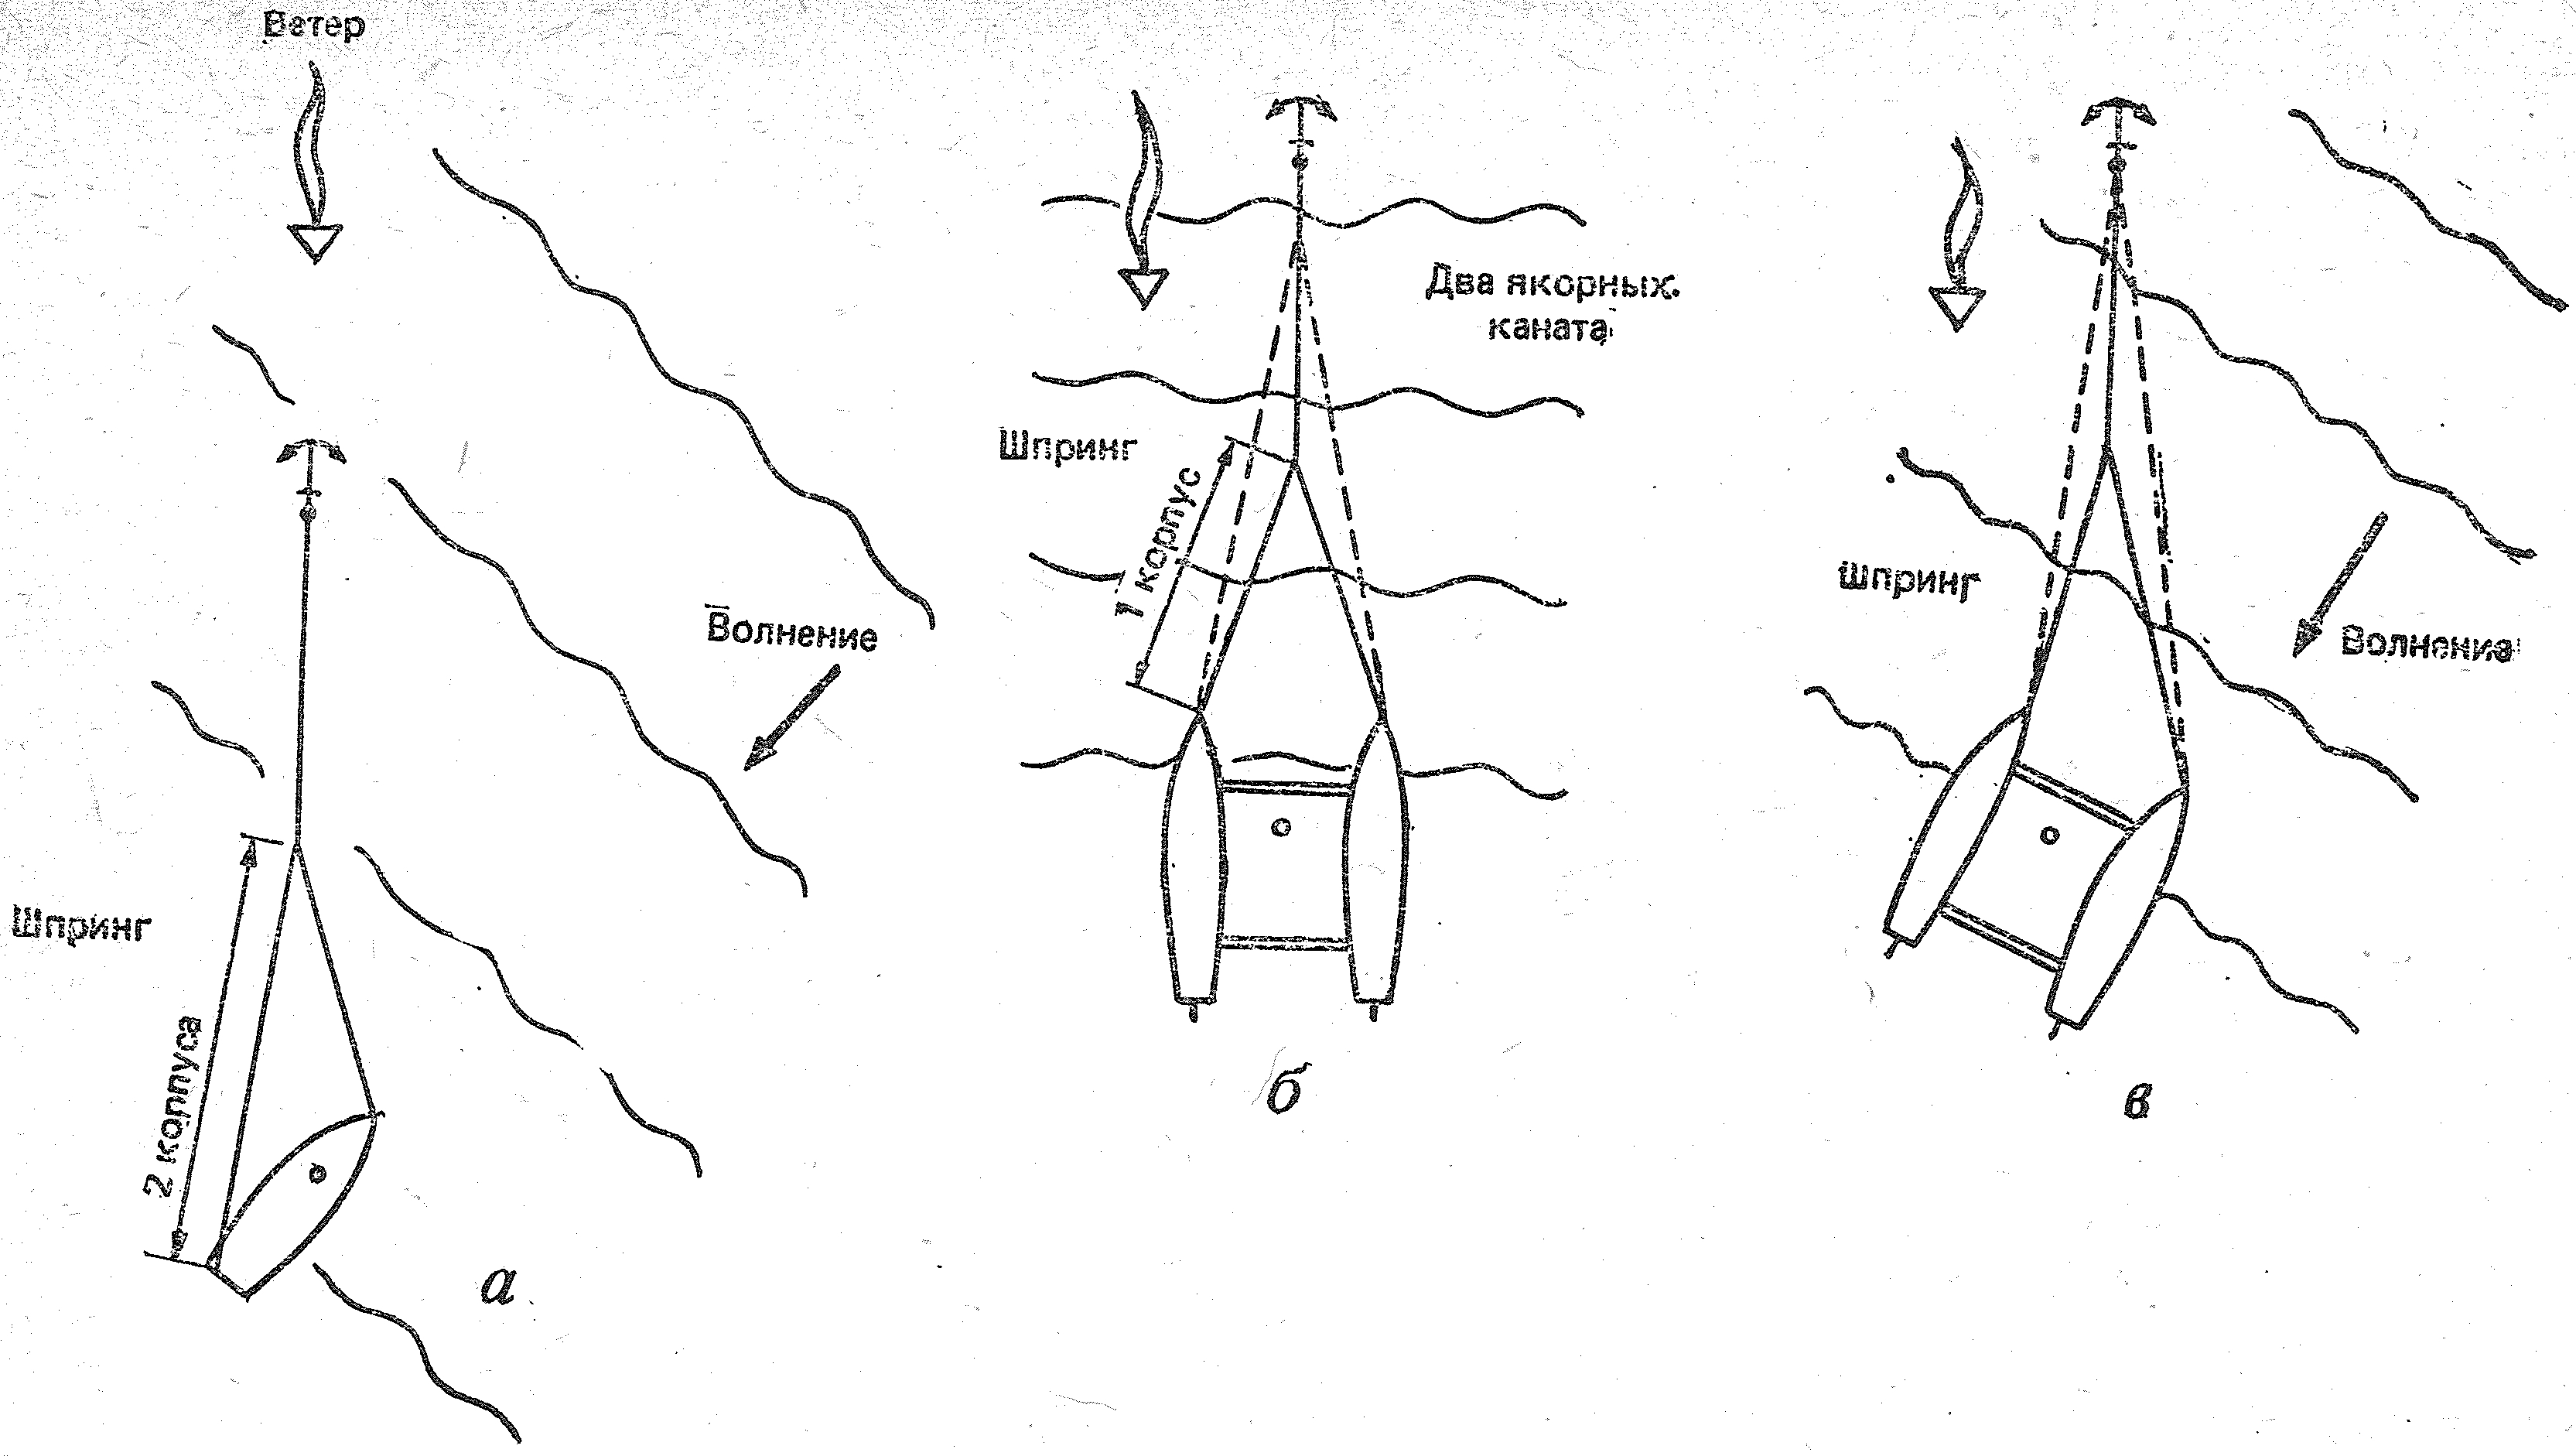
\includegraphics[scale=1.3]{0133P}
  \caption{Якорная стоянка на шпринге}
  \label{fig:133}
  \small
  \centering{}
  однокорпусной яхты (\textit{а}) и катамарана при разных направлениях ветра и волнения (\textit{б} и \textit{в})
\end{figure*}

Точно так же ставят на шпринг крейсерские катамараны. Катамараны ставят на якорь и таким образом: за рым одного якоря крепят сразу два каната, идущих на нос каждого корпуса (рис.~\ris{133}, \textit{б}, \textit{в}). 

\textbf{Постановка на два якоря.} К постановке на два якоря прибегают в том случае, когда хотят ограничить перемещения яхты на якорном канате в стеснённой акватории при переменных приливо\-/отливных течениях и непостоянных по направлению ветрах; или якорь приходится также отдавать, если яхта стоит кормой к берегу при сильном боковом ветре, на переменном, течении или во время шторма, когда одного якоря недостаточно для удержания судна на месте.

\begin{figure*}[htb]
  \centering{}
  \includegraphics[scale=1.3]{0134P}
  \caption{Стоянка на двух якорях способом <<фертоинг>> при ветрах переменных направлений}
  \label{fig:134}
\end{figure*}

Для ограничения перемещения яхты якоря отдают способом <<фертоинг>>. Если ожидается изменение направления ветра по всему горизонту, то якоря отдают так, чтобы угол между двумя якорными канатами составлял около 70\otdo 80\gr. В этом случае при заходе ветра на 90\gr один из якорей окажется за кормой яхты на расстоянии одного\-/двух корпусов (рис.~\ris{134}). Если же предполагается стоять на приливоотливном течении, то сначала отдают один якорь против течения, стравливают на двойную длину канат и отдают второй якорь. Затем добирают половину каната первого якоря и настолько же травят второй. Отданные якоря при штормовом ветре, перпендикулярном их линии, наверняка <<поползут>>.

Стоянка способом <<фертоинг>> не увеличивает держащую силу якоря во время шторма, так как яхта или все время стоит на одном якоре, или между якорями большой угол. Кроме того, при повороте ветра более чем на 180\gr якорные канаты перекрещиваются, образуя так называемый <<крыж>>.

Для того чтобы яхту не разворачивало при различных заходах ветра, например при стоянках в тесных гаванях или на реке, отдают один якорь с носа, другой с кормы.

Если яхта стоит перпендикулярно берегу на кормовых швартовых, при переменном течении или при сильных боровых ветрах, то отдают с носа два якоря симметрично линии \textit{ДП} или на ветер (против течения).

В шторм, когда держащей силы одного якоря при стравленном до жвака\-/галса якорном канате недостаточно, отдают второй якорь. На крейсерских яхтах это правый якорь увеличенного веса, на крейсерско\-/гоночных \--- верп, второй якорь отдают заблаговременно, то сначала насколько возможно добирают первый якорь, но так, чтобы не вырвать его, затем травят его канат отводят нос яхты в сторону, после чего отдают второй якорь. Затем оба якорных каната травят на нужную длину (рис.~\ris{135}, \textit{а}). Если же первый якорь <<пополз>>, то второй отдают прямо у борта, после чего травят только его канат. Если ожидается заход штормового ветра в известную сторону, то второй якорь завозят в сторону предполагаемого захода, но на меньшее расстояние, чем первый якорь. При заходе ветра, потравливая канат второго якоря, добиваются примерно одинаково его натяжения с первым (рис.~\ris{135}, \textit{б}).

Существуют три способа постановки на два якоря: с ходу, когда оба якоря отдают на малом ходу по линии, примерно перпендикулярной направлению ветра; с маневрированием на отданном якоре (стравливанием или подтягиванием) и с помощью туза. Для того чтобы против сильного ветра и волны завести верп, берут его вместе с канатом в туз, выходят на место, отдают верп и, травя трос, спускаются по ветру обратно к яхте. Более лёгкий якорь в большинстве случаев завозят на более дальнее расстояние. Для того чтобы против сильного ветра завести становой якорь с якорной цепью, вначале завозят верп (как мы уже говорили), а затем, вытягиваясь на верпе, завозят становой якорь. При этом половину якорь\-/цепи берут в туз. Сначала цепь потравливают с яхты, потом вторую половину травят с туза. Тяжёлый верп или становой якорь подвешивают за транцем туза, крепя его коротким концом-<<серьгой>> за среднюю банку.

Для того чтобы выбрать на тузе якорь (яхта при этом стоит на втором якоре или на буйке), заводят туз под якорь\-/цепь кормой к якорю, кладут цепь в вырез на транце туза и со средней банки выбирают её руками, одновременно потравливая немного якорь\-/цепь с яхты.

\textbf{Якорная стоянка в штормовых условиях.} Якорная стоянка безопасна лишь в том случае, если полностью закрыта от ветров и волнений всех направлений. Поэтому во время шторма не рекомендуется входить в незнакомые гавани или в открытые с моря заливы и бухты, из которых при заходе ветра невозможно выйти. Если же в силу сложившихся обстоятельств приходится штормовать на якоре, то необходимо принять все меры для предотвращения дрейфа якоря и навала на береговую отмель. 

Этими мерами являются: 
\begin{itemize}
\item уменьшение парусности корпуса и вооружения яхты, для чего необходимо опустить ноки гиков с парусами на палубу, плотно обтянуть или вообще убрать раздуваемые чехлы и т.\=,п.; 
\item отдача второго якоря; 
\item стравливание якорных канатов до жвака\-/галса; 
\item работа двигателя (если он есть) на переднем ходу; 
\item увеличение держащей силы якорей. 
\end{itemize}

Насколько осмотрительно и серьёзно следует относиться к выбору места якорной стоянки в шторм, показывает следующий пример.

{\small 13 августа 1976~г. польская яхта <<Отаго>> (стальной кэч, 29~тонн, 144\msq) отстаивалась на якорях от шторма в Баренцевом море за островом Медвежий. Резкий заход ветра с усилением не позволил своевременно сняться с якорей. Яхту сорвало с якорей и посадило на скалы. При попытке стащить <<Отаго>> с камней с помощью норвежского рыболовного судна яхта затонула на глубине 9~м.}

\begin{figure*}[htb]
  \centering{}
  \includegraphics[scale=1.3]{0135P}
  \caption{Стоянка на двух якорях в шторм}
  \label{fig:135}
  \small
  \centering{}
  \textit{а} \--- при постоянном направлении ветра; \textit{б} \--- при ожидающемся <<заходе>> ветра
\end{figure*}

\textbf{Повышение надёжности стоянки на якоре.} В шторм стоянка на двух якорях не всегда безопаснее, чем на одном якоре. Ветер и волнение сильно водят яхту, якорные канаты то рывком натягиваются, то ослабевают так, что в какие-то моменты практически работает только один якорь.

Для повышения держащей силы одного якоря есть три способа: 
\begin{itemize}
\item постановка на два якоря, укладываемых друг за другом способом <<гусёк>>; 
\item использование дополнительного груза, опускаемого на якорном канате; 
\item постановка на якорь с буйком. 
\end{itemize}

При постановке на якорь способом <<гусёк>> к тренту основного адмиралтейского якоря или к рыму якоря Данфорта крепят верп с помощью троса, длина которого примерно равна 1\otdo 1,5 глубины в данном месте. Сначала отдают верп, а затем и основной якорь и травят канат на нужную длину. Это самый надёжный из всех способов стоянки на якоре, пригодный для длительного отстаивания на рейдах.

При использовании дополнительного груза на петле или скобе, заведённой вокруг якорного каната, подвешивают какой-либо тяжёлый предмет или верп и с помощью линя длиной 1,5\otdo 2 глубины опускают вниз к якорю. В результате увеличивается провес якорного каната и удлиняется его горизонтальная часть, лежащая на грунте. Это увеличивает держащую силу якоря, ослабляет рывки и предохраняет его от вырывания из грунта.

Использование буйка при якорной стоянке существенно смягчает резкие рывки, которые неизбежны на большом волнении. Конец якорной цепи крепят к буйку, а яхта стоит на буйке с помощью <<серьги>>. В случае необходимости можно срочно сняться с якоря и перейти в другое, более безопасное место.

Большую опасность для яхты, отстаивающейся на якоре или на плавучем якоре в шторм, представляют удары гребней высоких волн. Для сглаживания водной поверхности и уничтожения гребней употребляют матерчатый мешок, набитый паклей, залитой маслом (например, машинным или соляровым), и прикреплённый к якорной цепи на расстоянии примерно 1\otdo 2 корпуса от яхты. 

\textbf{Техника снятия с якоря при неблагоприятных обстоятельствах.} На большинстве яхт, в особенности на крейсерско\-/гоночных, якорный канат выбирают вручную. В штормовой ветер у экипажа не хватает сил, чтобы его выбрать. Тогда делают это в такт килевой качке яхты: когда нос сходит с волны вниз \--- якорный канат ослабевает и слабину выбирают, когда нос поднимается на волне \--- якорный канат стопорят и держат до следующего ослабления каната . 

Если место для якорной стоянки недостаточно надёжно, а с моря пришёл внезапный шторм или шквал и для снятия с якоря уже нет времени, ставят штормовые паруса или даже один стаксель, отдают якорный канат за борт, оставляя якорь на грунте, и уходят в море. Поэтому при стоянке на открытом рейде никогда не следует убирать с палубы паруса (они всегда должны быть готовы к немедленной постановке).

Якорная цепь должна обязательно иметь жвака\-/галс с глаголь\-/гаком, и если для стоянки используется только часть цепи, то остатки её должны быть подняты из ящика на палубу, чтобы глаголь\-/гак был наверху и его легко можно было отдать. Иногда при стоянке в тесной гавани требуется срочно перейти на другое место, например, для ого, чтобы освободить место для большого судна, а якорь выбрать невозможно, так как над ним стоят позже пришедшие суда. Тогда можно либо заложить якорь\-/цепь на берегу, либо просто отдать её за борт, если якорь отдан с томбуем, либо, отдавая корь-цепь за борт, прикрепить к её концу буёк на буйрепе. 

В зависимости от характера якорных стоянок \--- на открытом рейде или защищённой гавани организуется различная вахтенная служба. На рейдовой стоянке на борту яхты должна находиться полная ходовая вахта, возглавляемая капитаном либо вахтенным начальником, обеспечивающая безопасность яхты и готовая в любой момент к снятию с якоря и переходу в другое место. На якорной стоянке в гавани, закрытой от волны и ветра, на орту яхты должна находиться стояночная вахта. На стоянке в оборудованных яхт\-/клубах, по договорённости руководством яхт\-/клуба, команда яхты может быть полностью отпущена а берег.

В обязанности вахтенной службы на якорной стоянке входит наблюдение за силой и направлением ветра, волнением, приливами и отливами, течением, а другими судами, за дрейфом яхты из-за <<ползущего>> якоря. При усилении ветра и волнения, а также с подъёмом воды вахтенные должны травить больше якорной цепи, зачастую вплоть до жвака\-/галса. Если этого недостаточно, нужно отдать или завести второй якорь, увеличить держащую силу якорей с помощью грузов, запустить двигатель и подрабатывать им на переднем ходу.

Если на рейдовой стоянке, несмотря на принятые меры, якоря не держат, то необходимо сняться и перейти в другое, более защищённое место или уйти в море и штормовать под парусами. Использовать шлюпку для завоза якорей и сообщения с берегом при рейдовой стоянке допускается при следующих условиях: волнение не представляет опасности для шлюпки, соблюдены нормы посадки, шлюпка снабжена спасательными приборами по числу находящихся в ней людей, назначен старший на шлюпке и, как правило, есть возможность визуального наблюдения за движением шлюпки лично вахтенным начальником на всем её пути. 

\section{Встреча шквала}

Шквал может прийти с любой стороны при любой погоде.

\begin{figure*}[htb]
  \centering{}
  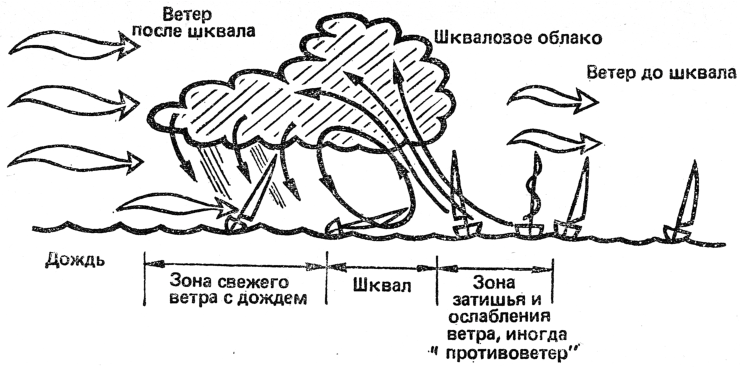
\includegraphics[scale=1.3]{0136P}
  \caption{Структура шквала}
  \label{fig:136}
\end{figure*}

В большинстве случаев его появление связано с прохождением фронтальных кучево\-/грозовых облаков или низких облаков с сильной внутри облачной конвекцией. В передней части такого облака движение восходящее, в центральной и тыловой \--- нисходящее. Они образуют в облаке и под ним горизонтальный вихрь (рис.~\ris{136}). Приближению такого облака с наветра предшествует затишье и кратковременный штиль, затем поворот ветра к облаку и его небольшое усиление (так называемый противоветер). Когда облако достигает зенита, следует первый удар шквала из-под облака. Затем приходит дождь со свежим ветром, после которого больше не засвежеет. С окончанием дождя устанавливается новый ровный ветер, иногда другого направления.

Характерным признаком приближения шквала в других случаях является так называемое шкваловое облако. Кроме того, на поверхности воды со стороны идущего шквала появляется тёмная полоса, а если идёт шквал силой более 6\otdo 7 баллов, то над водой видна быстро бегущая белая полоса бурунов и вихрей. При приближении шквала слышен шум приближающегося ветра и дождя. О силе шквала можно судить по характеру шквалового облака, его размерам и скорости перемещения.

Шквалы могут иметь и другую природу \--- они могут появляться при ясной, безоблачной погоде и даже с подветра. Шквал при ясной погоде называется <<белым шквалом>>. О его приближении можно судить только по бегущей тёмной или белой полосе воды. Во время шквала возможны резкие изменения направления ветра, что особенно опасно, когда шквал приходится принимать на полном курсе и ветер внезапно заходит с другого борта. Если шквал связан с прохождением холодного фронта, то ветер после него, как правило, поворачивает вправо. 

\textbf{Техника управления яхтой.} Обнаружив приближающийся шквал, следует разобрать бухты фалов, закрыть все люки, надеть спасательные жилеты и страховочные пояса. Дальнейшие действия зависят от силы шквала, типа вооружения яхты, курса относительно ветра, района и характера плавания.

При шквалах небольшой силы яхта продолжает идти своим курсом, экипаж внимательно следит за усилением шквала и его заходами. Шквал необходимо принимать только с наветра. Если он идёт с подветра, нужно заранее изменить курс, сделать поворот или даже убрать паруса.

Сильные шквалы встречают по-разному. В обычном плавании их лучше встречать на курсах бакштаг или бейдевинд, взяв рифы на гроте, заменив большие передние паруса на меньшие и обязательно убрать спинакер. Если нет времени на взятие рифов, то следует убрать грот и под одним стакселем встречать шквал на курсе бакштаг.

Когда во время гонки сильный шквал застаёт яхту на курсе бейдевинд, то надо немного увалиться и потравить гика\-/шкот. Кратковременный порыв можно встретить выйдя на ветер на грань заполаскивания парусов, чтобы только не потерять ход. Если шквал продолжительный, а уваливаться нежелательно, можно, не трогая стаксель шкотов и не меняя курса, потравить гика\-/шкот так, чтобы грот начало отдувать по передней шкаторине, и продолжать путь на задней шкаторине грота. Когда яхта идёт курсом галфвинд или крутой бакштаг, то на сильных шквалах следует уваливаться до полного бакштага, а при ослаблении ветра приводиться немного выше основного курса. При сильных шквалах, идущих зарядами один за другим, нужно уменьшить парусность.

\section{<<Человек за бортом!>>}

Основная задача капитана яхты или вахтенного начальника при падении человека за борт в кратчайший срок подойти к упавшему и взять его на борт. В книге невозможно дать рекомендации на все случаи жизни и предусмотреть все ситуации, которые могут возникнуть в конкретном плавании. Однако основные маневры необходимо отработать до автоматизма.

Независимо от того, каким курсом шла яхта к упавшему за борт, она должна подойти курсом бейдевинд, желательно с минимальным количеством поворотов и как можно скорее. На курсе бейдевинд всегда можно отрегулировать скорость яхты с помощью парусов, подбирая или потравливая их по мере надобности, а также сдрейфовать под ветер с растравленными шкотами. Если же подходить к упавшему в левентик, то при внезапных порывах ветра, его заходе или на крутой волне яхта может остановиться раньше времени и придётся делать повторный заход. Кроме того, следует иметь в виду, что подъём человека из воды может занять некоторое время, а в положении левентик судно стоять долго не может \--- через 10\otdo 15 секунд его обязательно увалит на тот или иной галс. На курсе же бейдевинд с растравленными шкотами, помогая рулём, можно яхту удерживать без хода значительно дольше. Поэтому специально планировать подход в левентик никогда не следует.

На большом волнении надо маневрировать так, чтобы не ударить плавающего в воде человека опускающимся с волны штевнем яхты.

\begin{figure*}[htb]
  \centering{}
  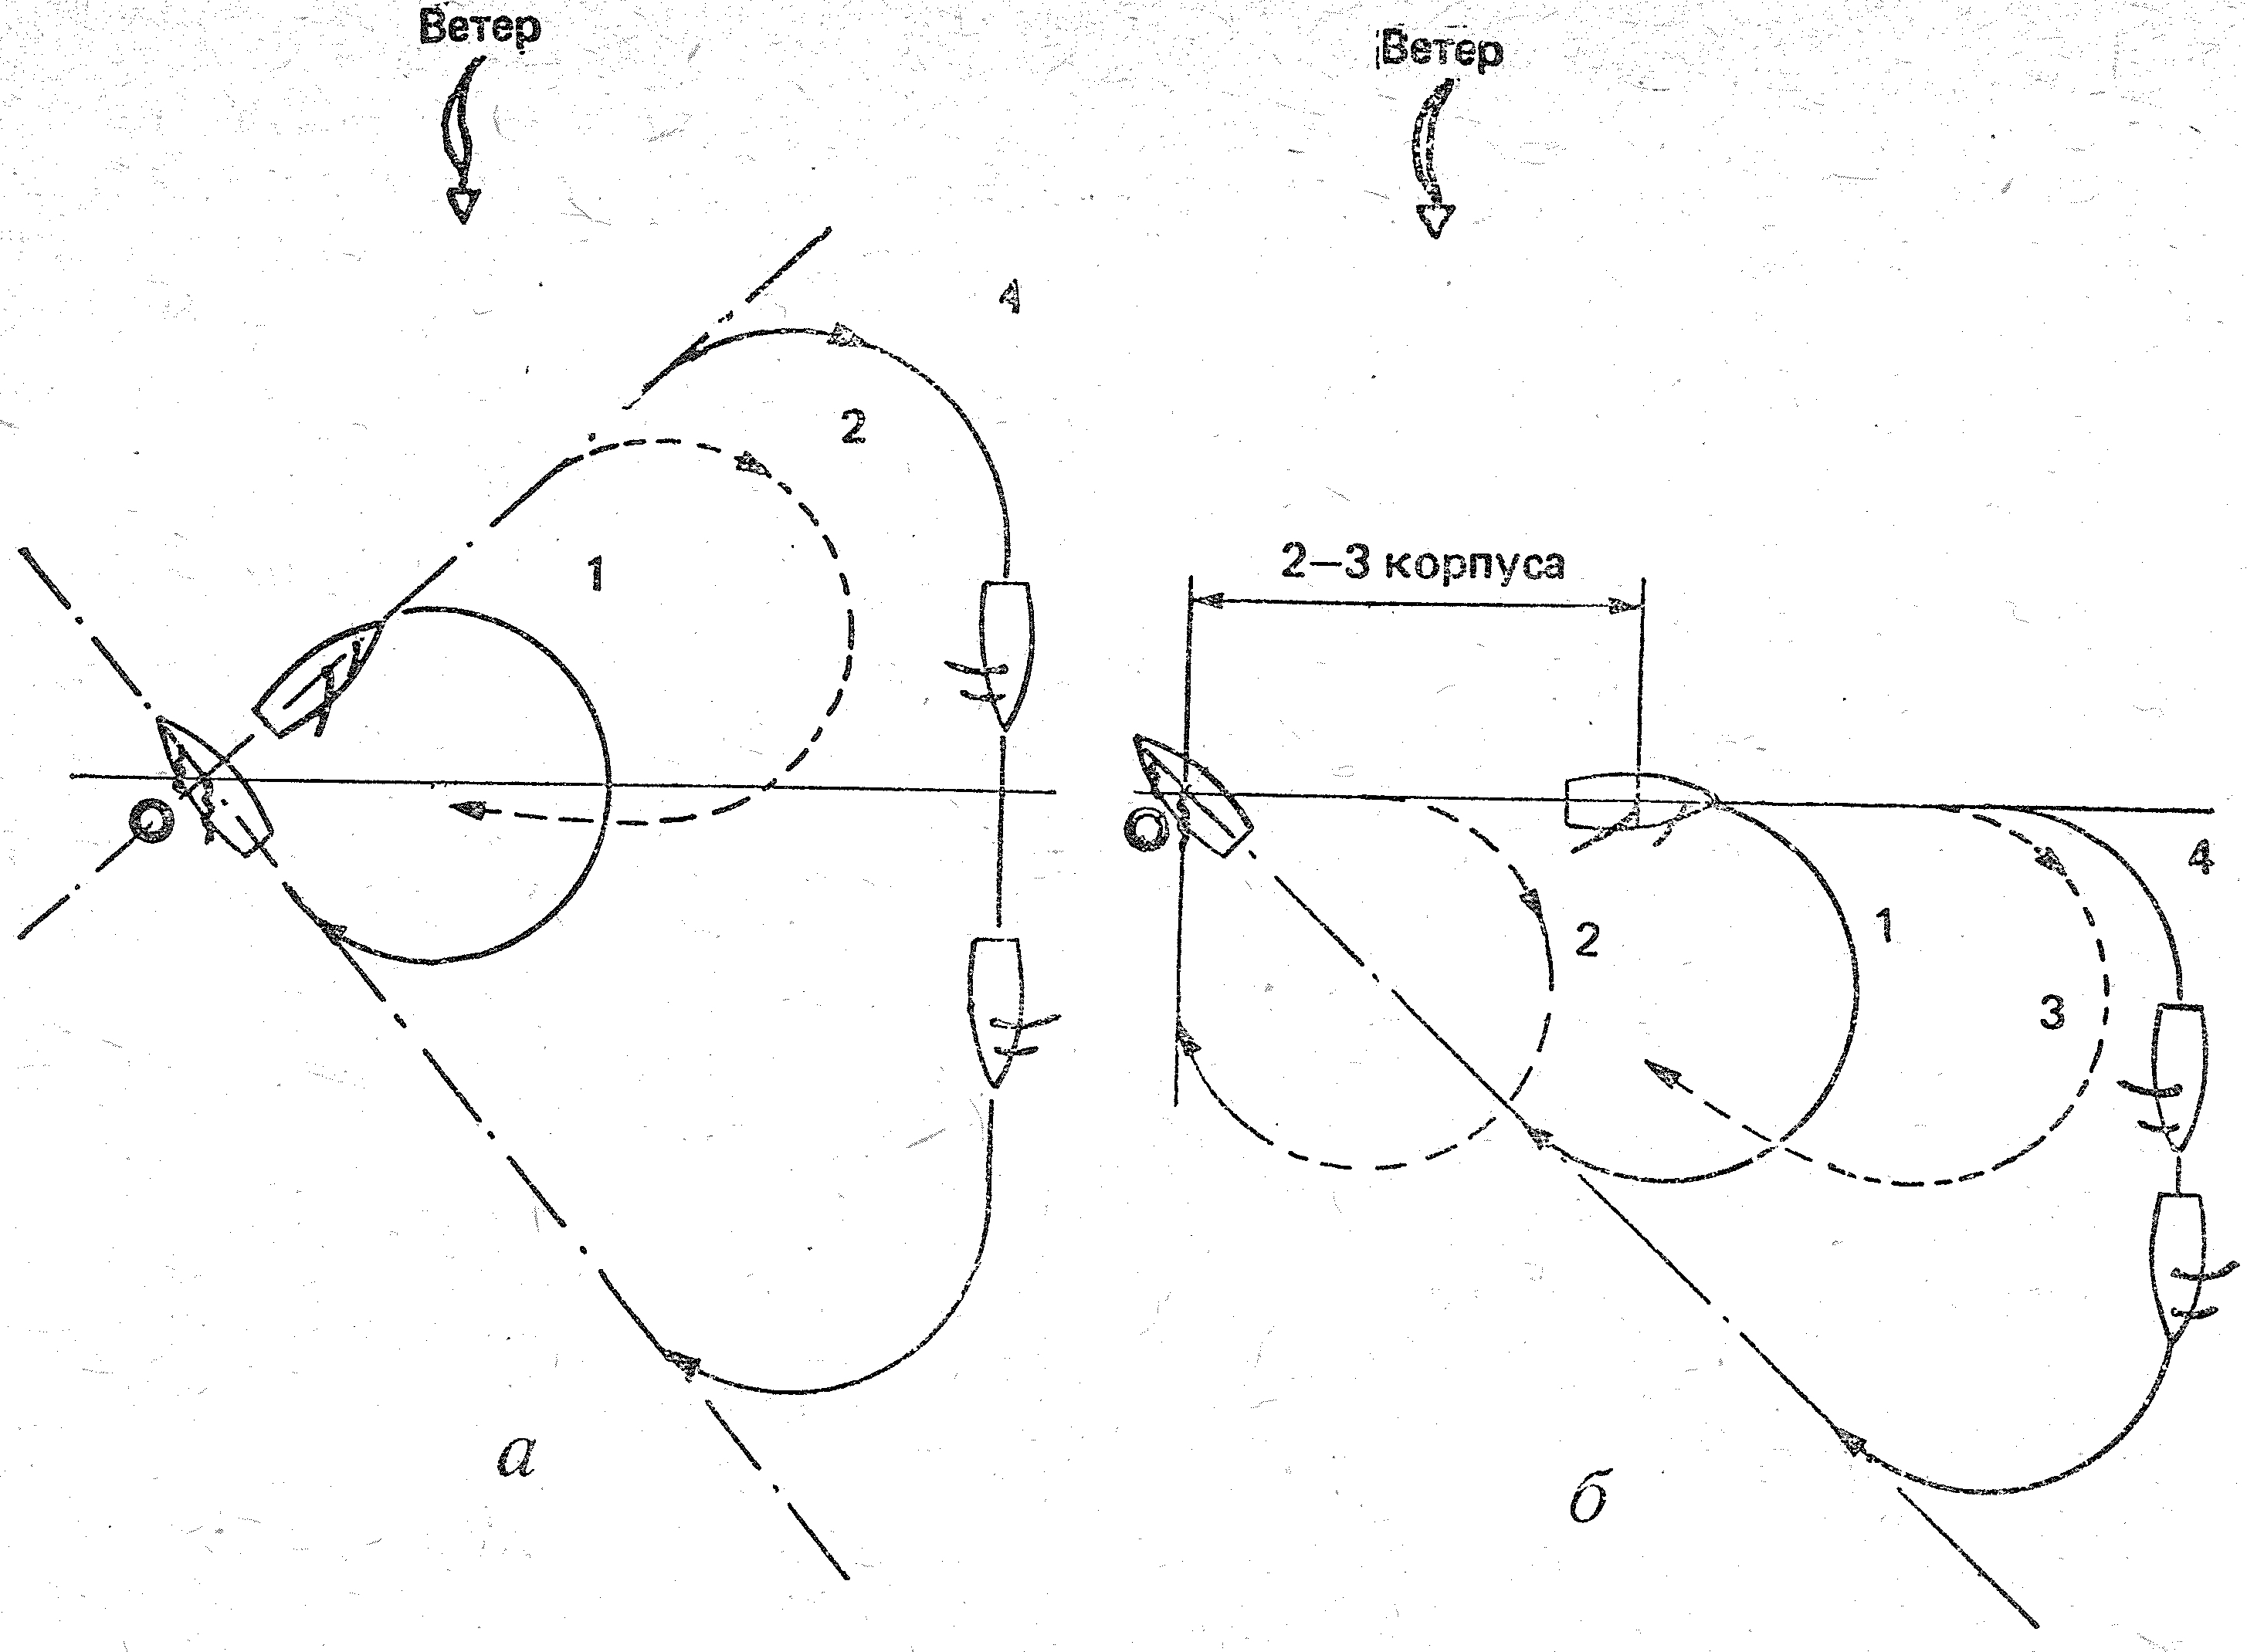
\includegraphics[scale=1.3]{0137P}
  \caption{Подход к упавшему за борт на курсе бейдевинд (\textit{а}) и галфвинд или крутой бакштаг (\textit{б}) с поворотом через фордевинд}
  \label{fig:137}
  \small
  \centering{}
  \textit{1} \--- в спокойную погоду; \textit{2} и \textit{3} \--- неправильно; \textit{4} \--- на сильном волнении в свежий ветер.
\end{figure*}

На килевых яхтах упавшего поднимают на борт только с подветренного борта в районе вант, на лёгких швертботах \--- только с наветренного борта или с кормы. Если человек упал за борт на курсе бейдевинд (рис.~\ris{137}, \textit{а}) в спокойную погоду, необходимо немедленно делать поворот фордевинд, так как из-за задержки поворота яхта может подойти к упавшему курсом галфвинд с большой скоростью (2). При падении человека на курсе галфвинд (рис.~\ris{137}, \textit{б}) поворот через фордевинд следует начинать, пройдя расстояние в 2\otdo 3 корпуса от упавшего тем же курсом. Если делать его позже (3), яхта может подойти к упавшему курсом полный бейдевинд с большим ходом, а если раньше (2) \--- просто не дойдёт до нужного места.

Если падение за борт произошло на курсе фордевинд или полный бакштаг (рис.~\ris{138}), необходимо, пройдя расстояние в 2\otdo 3 корпуса прежним курсом, привестись и сделать поворот оверштаг. Если поворот сделать раньше (2), то яхта подойдёт к упавшему курсом галфвинд, а если позже (3) \--- не дойдёт, до него. В свежий ветер или на большой волне для выполнения описанных маневров может понадобиться дополнительное время и место. Тут лучше немного потерять времени, но подойти точно и с первой попытки.

\begin{figure}[htb]
  \centering{}
  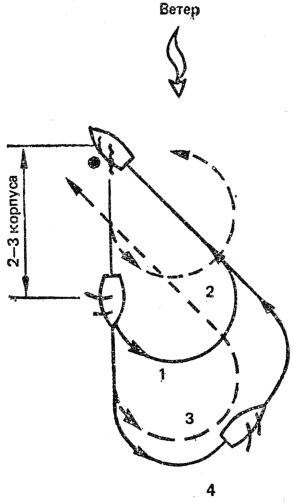
\includegraphics[scale=1.3]{0138P}
  \caption{Подход к упавшему за борт на курсе фордевинд или полный бакштаг с поворотом оверштаг}
  \label{fig:138}
  \small
  \centering{}
  \textit{1} \--- в спокойную погоду; \textit{2} и \textit{3} \--- неправильно; \textit{4} \--- на сильном волнении в свежий ветер
\end{figure}

Чтобы подобрать упавшего с курса бакштаг в спокойную погоду, сразу же необходимо либо привестись до галфвинда, либо увалиться на фордевинд (что ближе и удобнее) и затем сделать описанные маневры. Конкретно на сколько длин корпусов отходить от упавшего на разных курсах, когда делать поворот и ложиться на курс, когда травить шкоты при подходе к упавшему, зависит от многих причин, знать и предвидеть которые обязан каждый капитан, основываясь на собственном опыте. 

При плохой погоде в сильный ветер, когда есть риск сломать мачту или порвать паруса при повороте через фордевинд, с любого курса \--- от бакштага до бейдевинда упавшего подбирают с поворотом оверштаг (рис.~\ris{139}). В этом случае от места падения отходят на расстояние 3\otdo 4 корпусов, а иногда и больше, делают поворот оверштаг и сразу же уваливаются, травя гика\-/шкот, чтобы быстрее потерять запас наветренности. Придя на линию, ведущую курсом бейдевинд к упавшему, приводятся и добирают гика\-/шкот. Все маневры, начиная с подачи первой команды <<Человек за бортом!>> и до момента его подъёма из воды, должны сопровождаться чёткими и ясными командами капитана. Человек, ведущий наблюдение за упавшим, должен постоянно, через небольшие промежутки времени, докладывать капитану по установленной форме, например: <<Упавший справа, 45\otdo 30 метров>>, <<Слева у вант, 2 метра>> и т.\=,п. Встречаются необычные ситуации, в которых могут быть применены другие маневры. Если падение человека за борт произошло на курсе фордевинд или бакштаг и с наветренного борта находится препятствие, например берег или отмель, то подходят к упавшему с двумя поворотами, сначала пройдя расстояние в 2\otdo 3 корпуса, через фордевинд, а затем \--- оверштаг (рис.~\ris{140}).

При падении человека за борт ночью или при плохой видимости немедленно привестись или увалиться до галфвинда, заметить курс по компасу и идти им по громкому отсчёту одного из членов экипажа в течение 10\otdo 15~сек., затем сделать поворот и возвращаться противоположным курсом по компасу в течение того же времени. Место упавшего человека определяют по светящемуся буйку, сброшенному в воду в момент падения за борт, звуку свистка или крику человека (рис.~\ris{141}). Ночью при подходе к месту падения и поиске необходимо использовать белые осветительные ракеты. Обнаружив человека, следует заранее (если это нужно) несколько увалиться, чтобы подойти к нему курсом бейдевинд с растравленными шкотами. Когда с первой попытки найти человека не удаётся, следует ходить в предполагаемом районе падения галсами по времени, перекрывая все большую и большую площадь как на ветер, так и под ветер. При падении человека за борт на курсе фордевинд под спинакером нужно, убрав спинакер, возвращаться к месту падения в лавировку короткими галсами, чтобы все время просматривался генеральный путь яхты к упавшему.

\begin{figure*}[htb]
  \centering{}
  \includegraphics[scale=1.3]{0139P}
  \caption{Подход к упавшему за борт в свежий ветер с поворотом оверштаг}
  \label{fig:139}
  \small
  \centering{}
  на курсах полный бакштаг, бакштаг около 135\gr к ветру и крутой бакштаг (\textit{а}); на курсах бейдевинд и галфвинд (\textit{б})
\end{figure*}

Может оказаться, что на борту яхты было только два человека и один из них оказался за бортом. Если яхта шла курсом бейдевинд, необходимо бросить упавшему круг и положить руль до отказа под ветер, прижав его в этом положении, и, не трогая шкотов, быстро приготовить бросательный конец; в момент перехода грота на другой борт перезаложить бакштаги и перенести стаксель под ветер, выбрав его сразу втугую. После этого остаётся только ждать, когда упавший человек окажется по носу яхты, и в этот момент положить руль прямо. Как только упавший поравняется со штевнем, следует отдать все шкоты, прихватить чем-либо румпель в ДП и бежать к вантам с бросательным концом. Это самый быстрый и точный способ подхода к упавшему на курсе бейдевинд даже на больших яхтах при ветре силой 3\otdo 4~балла, т.\=,е. когда удаётся увалить яхту до курса фордевинд, не травя гика шкотов. В подобном же случае можно подойти к упавшему с дрейфом: на курсе бейдевинд следует, бросив круг, сразу увалиться, не трогая шкотов, примерно до галфвинда, пройти расстояние в 3\otdo 4 корпуса и сделать поворот оверштаг, перезаложив при этом только бакштаг. Яхта ляжет в дрейф. Рулём вначале необходимо увалить яхту, чтобы потерять излишнюю наветренность, а затем привестись и ждать, когда она сдрейфует к упавшему (рис.~\ris{142}, \textit{а}). Такой подход не самый быстрый, но, поскольку при этом почти не надо работать со шкотами, он незаменим, если на борту остаётся только один человек, да к тому же не очень опытный. Подойти к упавшему, таким образом, можно с любого курса (рис.~\ris{142}, \textit{б}). Поворот оверштаг для постановки яхты в дрейф в этих случаях следует делать примерно на расстоянии 1 корпуса наветреннее от упавшего в воду. 

\begin{figure}[htb]
  \centering{}
  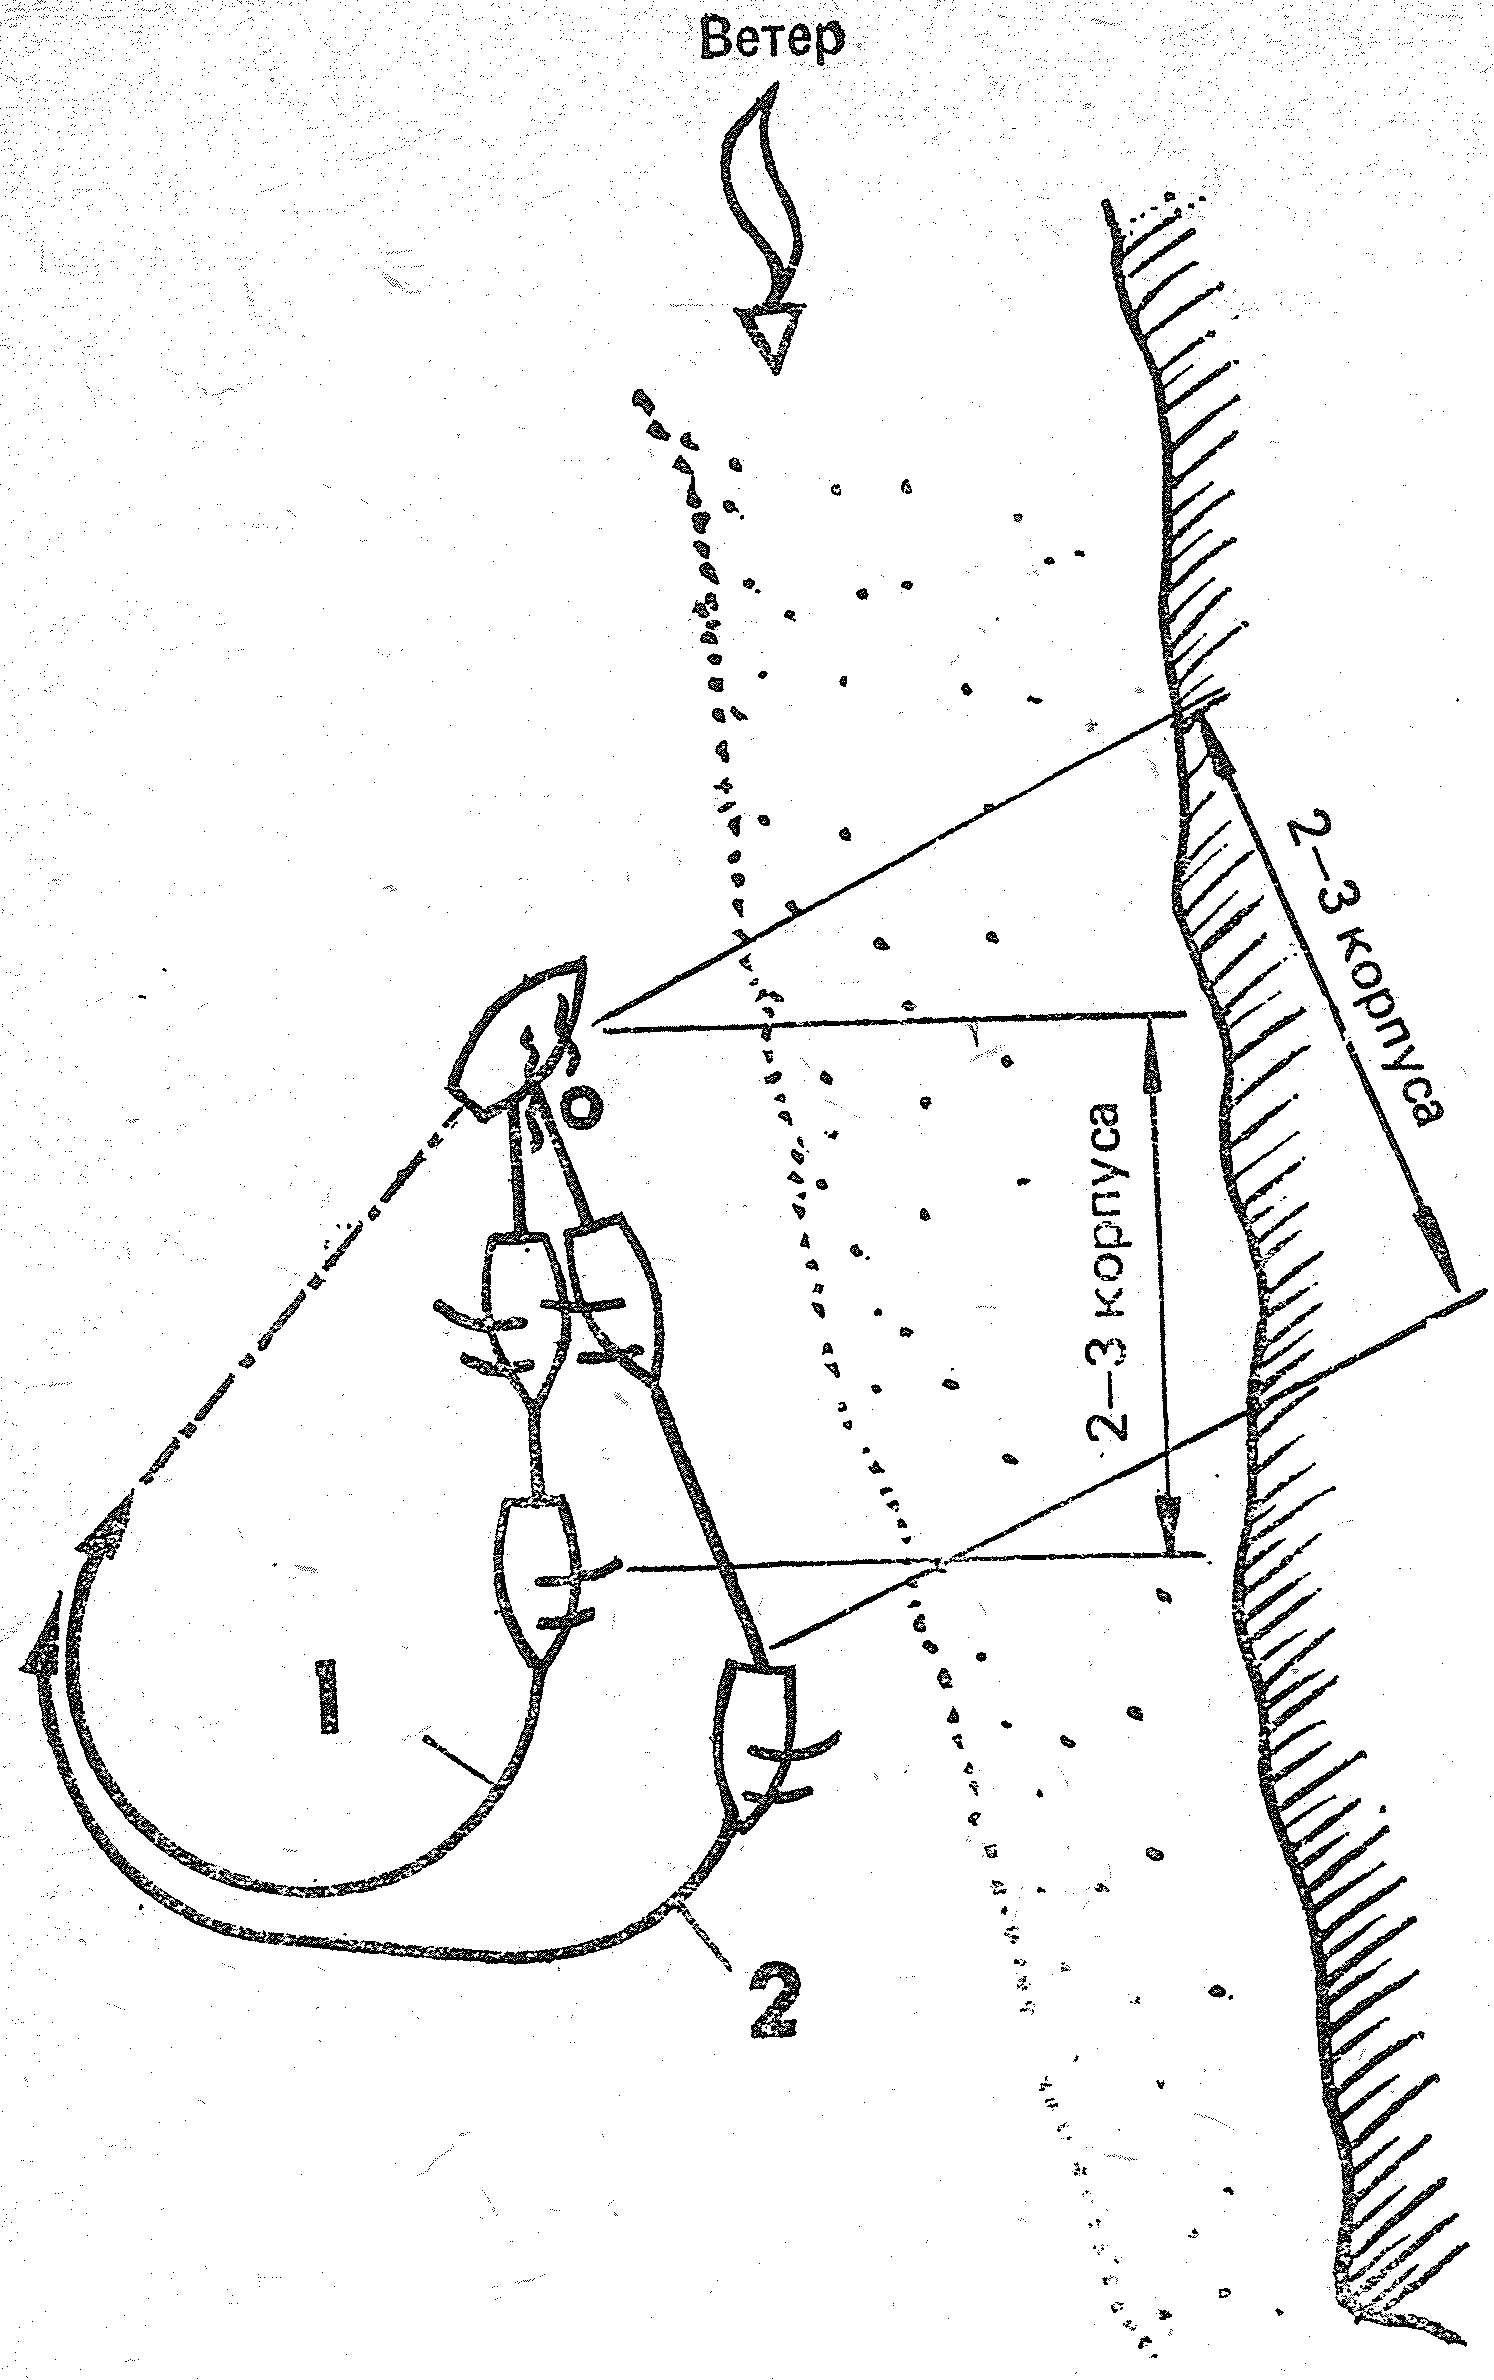
\includegraphics[scale=1.3]{0140P}
  \caption{Подход к упавшему за борт с двумя поворотами у препятствия}
  \label{fig:140}
  \small
  \centering{}
  \textit{1} \--- на курсе фордевинд; \textit{2} \--- на курсах галфвинд и бакштаг
\end{figure}

Разные типы яхт дрейфуют по-разному, в зависимости от формы корпуса и типа вооружения. Одни хорошо лежат в дрейфе с туго выбранным гика шкотом, другие \--- с немного потравленным. Если яхта сдрейфует ниже упавшего за борт, то достаточно подобрать гика\-/шкот, если выше, то побольше растравить. При неудачном подходе стаксель переносят под ветер и маневр повторяют. При маневрировании с дрейфом упавший все время находится в поле зрения рулевого яхты, на большой волне яхта подходит к нему не штевнем, а бортом.

\section{Оказание помощи судну, терпящему бедствие}

Согласно ст.~53 КТМ и правилам 58~ППС-77, капитан яхты обязан оказать помощь любому судну или лицу, терпящему бедствие, если он может сделать это без опасности для своей яхты и её экипажа.Подходя к судну на открытой воде, необходимо в первую очередь подобрать всех людей, оказавшихся в воде, начиная с самого подветренного. Тех, кого не удаётся подобрать сразу, нужно обеспечить спасательными средствами.

Для снятия людей с аварийной яхты подходят носом против ветра к её оконечностям, остерегаясь плавающих вокруг обломков рангоута. При большом волнении вплотную к ней подходить не следует, снимать людей нужно с помощью концов.

Для взятия аварийной яхты на буксир рекомендуется проходить на малой скорости на некотором расстоянии вдоль борта, свободного от обломков рангоута, буксирный конец подавать с наветренной яхты. В свежий ветер и на большой волне для облегчения заводки буксирного троса полезно с аварийной яхты заранее стравить под ветер тонкий проводник (с буйком, кругом или пустой канистрой), который сможет подобрать из воды буксирующее судно. В качестве буксирного троса применяются синтетические тросы, обладающие высокой прочностью, эластичностью и упругостью, что очень важно при буксировке на сильной волне. 

\textbf{Буксировка аварийного судна.} В открытом море на большой волне аварийное судно буксируют за кормой на буксирном тросе, длину которого выбирают равной или кратной длине волны по направлению курса, чтобы обе яхты одновременно сходили и поднимались на гребень. Длина буксира не должна быть меньше двух длин корпусов наибольшей яхты. На обоих яхтах буксирный трос крепится за мачту либо за швартовные утки или шпили, если они имеют достаточно мощные подкрепления. Буксирный трос нельзя проводить через полуклюзы, так как на яхтах они слабые и их обязательно вырвет. 

\begin{figure}[htb]
  \centering{}
  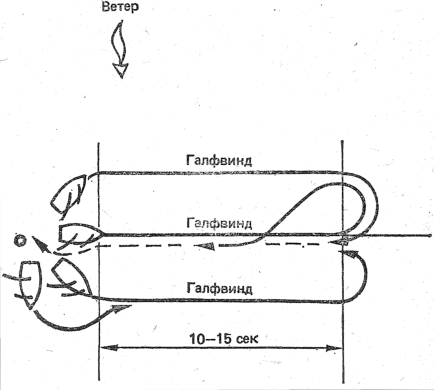
\includegraphics[scale=1.3]{0141P}
  \caption{Подход к упавшему за борт ночью или в плохую видимость}
  \label{fig:141}
\end{figure}

Во избежание смятия металлической мачты или перетирания деревянной её предварительно обматывают парусиной и обкладывают деревянными планками. Если трос на буксирующей яхте крепится за мачту, то в районе кокпита рулевого должна быть сделана оттяжка троса к борту. Чтобы буксирный трос не <<гулял>>, на, корме буксирующей яхты и на носу буксируемой его крепят специальными стропками надёжным оковкам или проводят через петлю, заведённую вокруг штевня и кормового подзора. Чтобы трос не перетирался на гакаборте и ватервейсе его в этом месте обматывают парусиной.Если на буксируемом судне трос закладывать не за что, то его крепят с помощью браги, обнесённой вокруг корпуса яхты примерно на половине высоты борта. От сползания вниз она удерживается достаточным количеством стропок, заложенных за обушки и утки на палубе. Буксирный трос крепят буксирным узлом, и на обеих яхтах около него ставят вахтенного матроса, чтобы следить за креплением, беречь трос от перетирания, выбирать слабину и отдавать его по команде капитана.

Когда яхта под парусами берет другую на буксир, то все маневры по буксировке выполняют с потравленными шкотами. Лишь после того как буксирный трос обтянется и буксируемая яхта <<придёт на буксир>>, можно плавно подобрать шкоты и лечь на курс. Если яхты имеют одинаковое водоизмещение, буксировка практически удаётся не круче галфвинда; когда же буксирующая яхта имеет существенно меньшее водоизмещение, то в отсутствие большого волнения можно даже подняться на ветер. Это следует иметь в виду при буксировке аварийной яхты в укрытие.

Буксируемая яхта должна идти в кильватер буксирующей. При поворотах она должна стараться идти по наружной стороне кильватерной струи, чтобы помогать повороту буксирующей яхты. Перед этим выбирается слабина троса, но так, чтобы не мешать повороту буксира. На волне, в очень сильный или в очень слабый ветер поворот оверштаг с буксируемой яхтой за кормой не удаётся. Лучше сделать поворот фордевинд по очень пологой циркуляции.

\begin{figure*}[htb]
  \centering{}
  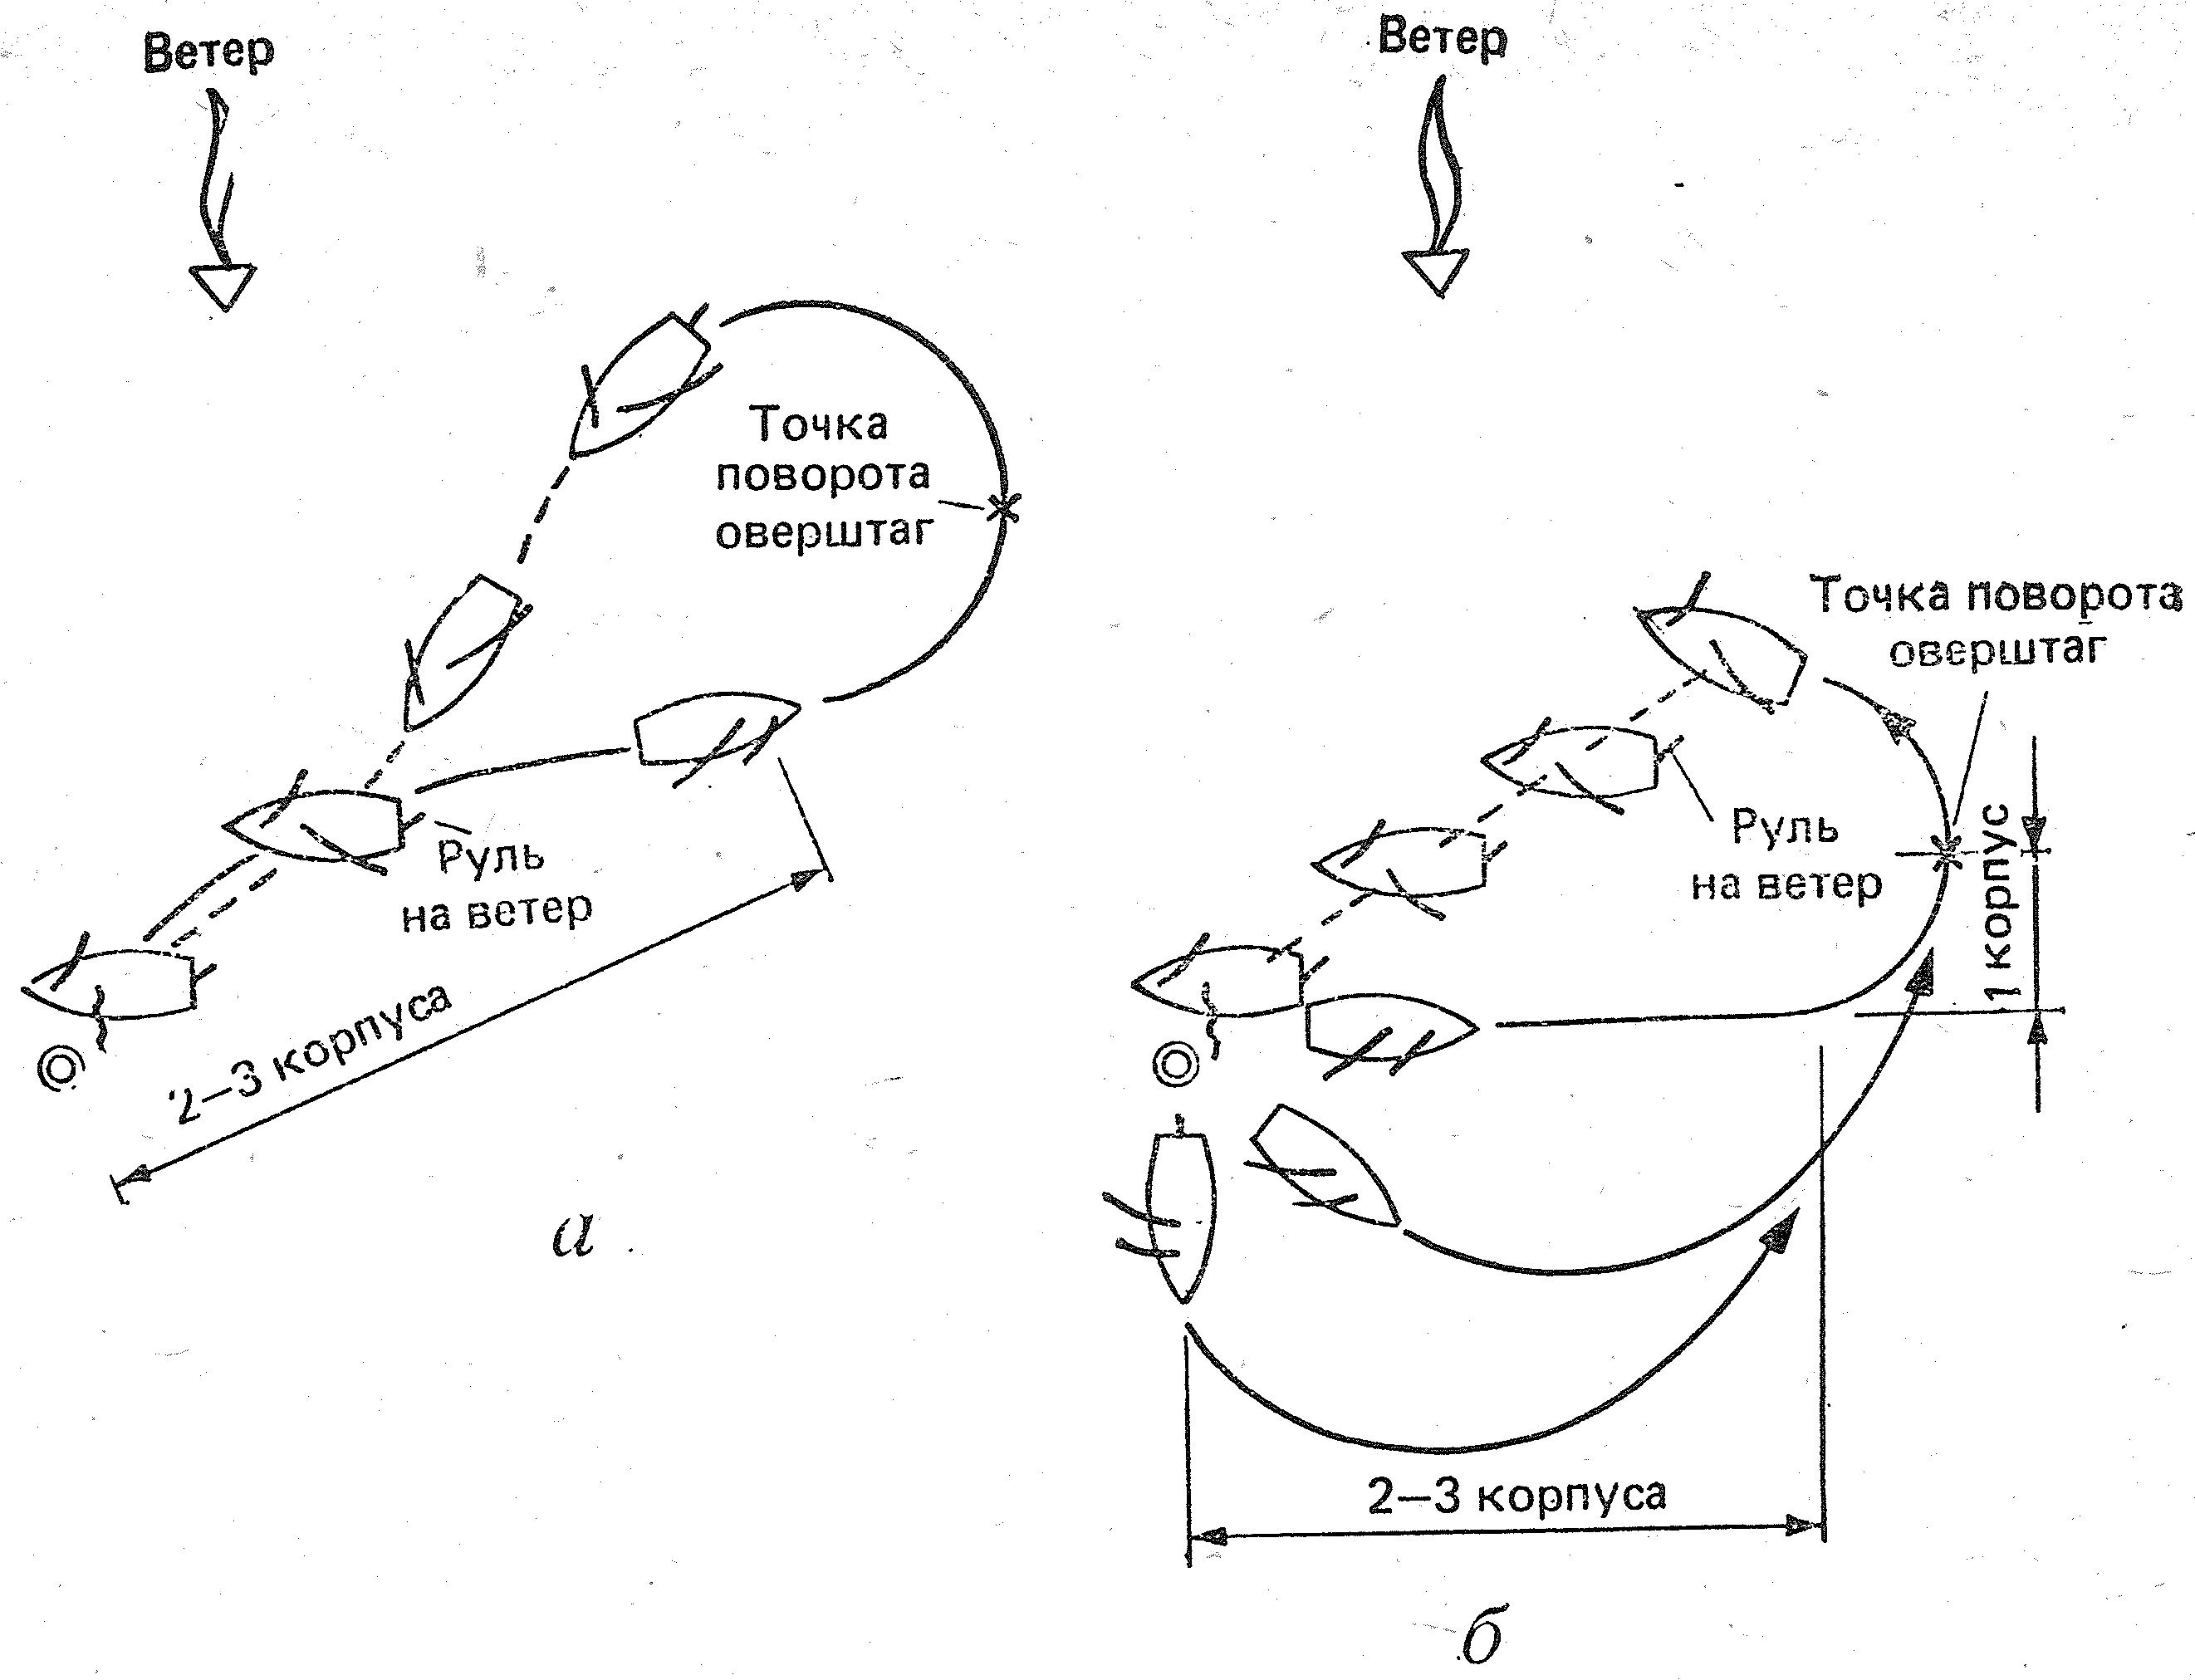
\includegraphics[scale=1.3]{0142P}
  \caption{Подход к упавшему за борт с дрейфом}
  \label{fig:142}
  \small
  \centering{}
  на курсе бейдевинд (\textit{а}) и на курсах галфвинд, бакштаг и фордевинд (\textit{б})
\end{figure*}

Буксировка яхты под мотором технически намного проще, чем под парусами. Но следует особо тщательно следить за появлением слабины буксирного троса, которую надо немедленно выбирать, а при натяжении троса плавно его травить. Если этого не делать, трос рано или поздно попадёт под корму буксирующей яхты и намотается на винт.Если на большой волне аварийная яхта снимается с якоря с помощью буксирующего судна и под ветром есть чистая вода, необходимо сначала выбрать якорь, увалиться под рангоутом по ветру и затем принять или подать буксир на буксирующее судно, идущее параллельным курсом. Если под ветром в непосредственной близости берег, то следует, не выбирая якоря, завести на буксирующее судно буксирный трос и затем отдать за борт якорный канат (привязав к его концу буёк).

Не рекомендуется выбирать якорь при заведённом буксирном тросе, так как это может привести к аварийной ситуации. Так, если якорь выбирать с натянутым буксирным тросом, то яхта может не пройти над ним, и его тогда нельзя будет вырвать. Если же при выборке якоря буксирный трос будет иметь большую слабину, то он может намотаться на винт судна либо запутаться вокруг плавника и пера руля яхты.

При буксировке на буксирном тросе всегда должны работать самые опытные матросы, так как петли троса, образующиеся на слабине, представляют серьёзную опасность для человека при внезапном рывке буксира. 

\section{Аварии на яхте, меры их предупреждения и ликвидации}

Обрыв такелажа. Если на ходу лопнул или отдался штаг, то необходимо, потратив гика- и стаксель шкоты, увалиться на фордевинд, после чего сначала завести фальшивый штаг (например, из запасного стаксель фала), а затем заменить (починить) сломанную деталь.

Если лопнула или отдалась наветренная ванта, бакштаг или выскочила наветренная краспица, следует немедленно потравить шкоты и лечь на другой галс (или в дрейф) с поворотом оверштаг, затем заняться ремонтом повреждения. Если наветренная ванта отдалась на курсе фордевинд, то необходимо сделать поворот фордевинд и привестись на острый курс.

Если лопнул ахтерштаг, то следует привестись на острый курс и выбрать гика\-/шкот, после чего завести фальшивый ахтерштаг (например, из топенанта).

Можно заменить повреждённые снасти на ходу, когда есть запасные ванты и бакштаги. Во время этой операции площадь парусов уменьшают до предела и ложатся на курс, при котором повреждённая снасть находилась бы под ветром.

Если лопнул или выхлестнулся гика-шкот, то подветренным бакштагом подтягивают гик, приводятся до положения левентик, накидывают на нок гика петлёй конец, который крепят к кормовым уткам. Затем, увалившись на нужный курс, заводят новый гика-шкот.
Если лопнул подветренный стаксель-шкот, то возможны следующие варианты: 
\begin{itemize}
\item сделать поворот оверштаг и заменить шкот на другом галсе; 
\item перенести наветренный шкот под ветер, а затем заменить лопнувший; 
\item подобрать наветренный шкот и заменить лопнувший подветренный шкот (годится только для стакселей); 
\item убрать стаксель (геную) для замены шкота. 
\end{itemize}

\textbf{Поломка мачты.} При поломке мачты необходимо убедиться, нет ли пострадавших, не оказался ли кто-нибудь за бортом, и оказать им необходимую помощь, после чего поднять на борт обломки мачты и такелажа и снять с них паруса.

Если сломалась металлическая мачта и поднять её на борт невозможно, то при сильном волнении нужно освободиться от мачты, обрубив стоячий такелаж. Затем дать яхте ход. Без мачты резко изменяется момент инерции яхты \--- её начинает резко и порывисто качать, что плохо отражается на работоспособности команды.

Когда мачта ломается выше нижних краспица, а основные ванты целы, то на остатках мачты, предварительно укрепив её ложным стоячим такелажем, можно поставить штормовой стаксель и трисель. Когда же она ломается у пяртнерса, то в качестве фальшивой мачты можно использовать спинакер\-/гик, гик или футштоки, раскрепив её как минимум двумя вантами, штагом, ахтерштагом и установив наверху два блока для фалов.

\textbf{Поломка руля.} Если сломан баллер или потеряно перо руля, то необходимо лечь в дрейф под парусами или встать на плавучий якорь и сделать аварийный руль. Для этого используют два футштока или спинакер\-/гика, закрепив между ними какую-нибудь доску, например полик. К доске крепят два браса, заводят их на шпили шкотовых лебёдок правого и левого бортов. Устройство устанавливают на корме яхты под углом 30\otdo 45\gr к горизонту с помощью мощного бензеля и оттяжки, проведённой к обушкам на палубе. Регулируя натяжение брасов, устанавливают необходимое положение временного руля относительно \textit{ДП} яхты. Это самая надёжная конструкция временного руля для управления яхтой в свежую погоду.

Многомачтовыми яхтами с длинной килевой линией и большим количеством парусов можно управлять с помощью парусов. Потравливая или выбирая шкоты носовых и кормовых парусов, можно регулировать курс яхты в довольно широких пределах. 

\textbf{Борьба с течью.} При появлении течи немедленно нужно организовать откачку воды из трюма, причём чаще всего самая эффективная откачка \--- с помощью обычных вёдер. Если течь обнаружена в районе ватерлинии или выше, надо сменить галс так, чтобы место течи оказалось на наветренном борту.

Для ликвидации пробоины или течи используют чехлы, тряпки, одеяла, деревянные подушки, нарезанные в размер шпации и обернутые парусиной клинья. Надо стараться заделать пробоину изнутри. Иногда приходится заводить пластырь снаружи корпуса, для чего можно использовать один из штормовых стакселей. На яхтах с металлическим или пластмассовым корпусом для окончательной заделки пробоины лучше всего поставить цементный ящик. Бетон приготавливают из цемента марок 400 или 600, смешивая его с песком в отношении от 1\=,:\=,3 до 1\=,:\=,1. В смесь доливают пресную воду и перемешивают до консистенции густого теста. Для ускорения схватывания бетона в воду добавляют 10\,\% жидкого стекла или 5\,\% технической соды. Для прочности заделать в бетон арматуру. 

\textbf{Борьба с пожаром.} При возникновении пожара ходовая вахта уваливает судно на курс фордевинд, чтобы уменьшить крен яхты и скорость вымпельного ветра, раздувающего огонь, а аварийная команда устанавливает, что горит, и тушит пожар, предварительно перекрыв топливные магистрали, газ и отключив электроэнергию. Горящий бензин и электрооборудование под напряжением можно тушить только углекислотными огнетушителями (ОУ-2 или ОУ-5), все остальное тушат водой или любой плотной тканью (одеялом, чехлом и т.\=,п.).

Наибольшую опасность на яхте в пожарном отношении представляют бензиновый двигатель и газовый камбуз. Поскольку размеры большинства яхт обычно не позволяют выделить для них отдельных отсеков, то следует обеспечить герметичность бензобаков и газовых баллонов, удалить их от соседства с открытым огнём и источниками тепла. Желательно вынести их из жилых помещений. Яхта должна иметь хорошую вентиляцию. 

\begin{figure*}[htb]
  \centering{}
  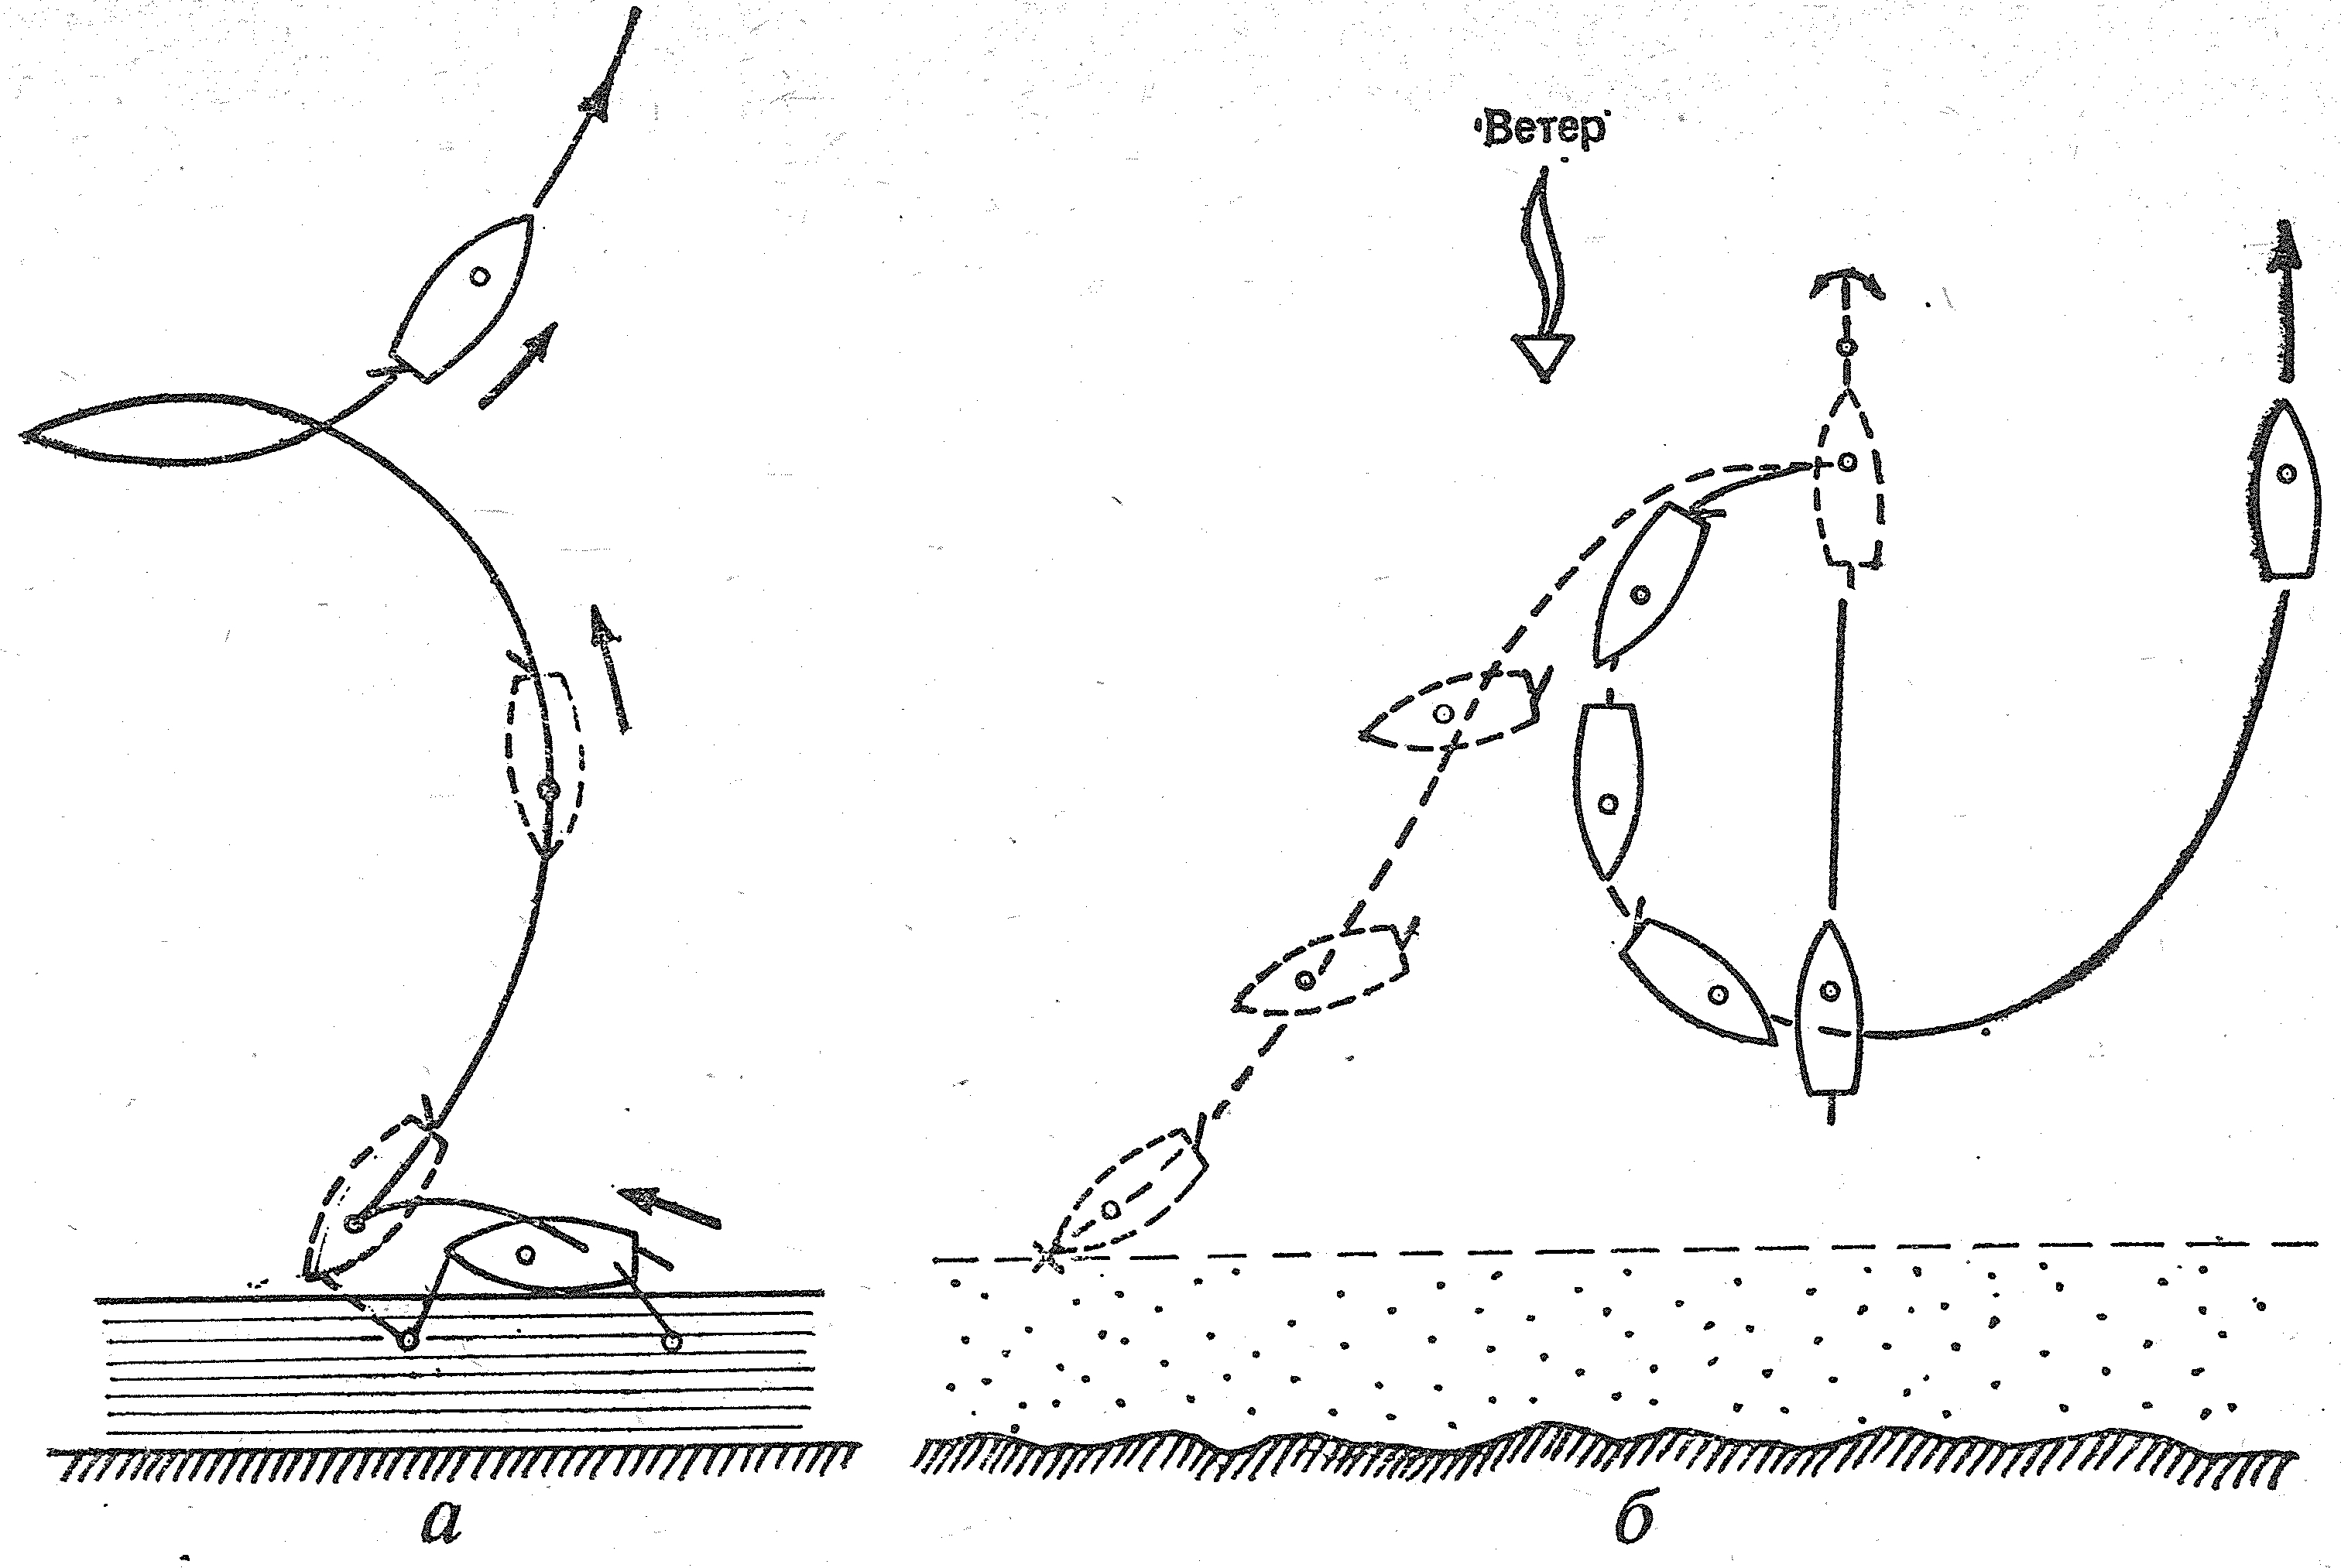
\includegraphics[scale=1.3]{0143P}
  \caption{Отход от стенки (а) и снятие с якоря (б) яхты под мотором при навальном ветре}
  \label{fig:143}
\end{figure*}

\textbf{Управление под мотором.} Поскольку современные яхты имеют большую боковую поверхность плавниковых фальшкилей, направление вращения винта оказывает небольшое влияние на их управляемость на ходу. Тем не менее у яхт с маломощными моторами некоторые особенности управления существуют. Так, при навальном ветре отход от стенки на шлюпе \sfrac{3}{4} легче выполнять кормой на ветер (рис.~\ris{143}, \textit{а}).

Снимаясь с якоря у подветренного берега при штормовом ветре, после того как якорь будет вырван, необходимо сначала увалиться и разогнать яхту, а затем привестись к ветру. Если этого не сделать, то маломощный двигатель может не <<выгрести>> против ветра \--- яхту снесёт на мель (рис.~\ris{143}, \textit{б}). Следует учитывать и то, что на заднем ходу при работающем моторе яхтой управлять плохо.
Для срочной остановки яхты в узком фарватере необходимо включить полный ход назад и немного переложить руль в сторону вращения винта. 

\section{Особенности крейсерских гонок}

Крейсерские гонки, по существу, являются самостоятельным видом спорта и имеют ряд принципиальных отличий от парусных гонок на олимпийской дистанции. Олимпийские гонки проводятся на очень ограниченной акватории в течение короткого времени (несколько часов), при этом в основном ведётся ближняя тактическая борьба, при которой особо большое значение приобретают взятие старта, огибание знаков и т.\=,п. Крейсерские же гонки проходят на длинных дистанциях, охватывающих различные районы моря с разными ветровыми и навигационными условиями; длятся они по несколько суток. Поэтому здесь на одно из главных мест выходят мореходное искусство и общая морская подготовка.

Тактика гандикапных гонок часто основывается на выборе оптимального маршрута и быстрейшем прохождении дистанции, в то время как в классной гонке успех в значительной степени решает умение контролировать противника от старта до финиша. Тактика крейсерских гонок во многом зависит от свободы, которую имеет яхта в выборе своего маршрута. Здесь могут быть два наиболее общих случая: когда маршрут частично или полностью регламентирован по условиям гонки и когда ничто не влияет на выбор пути. 

\textbf{Форсирование парусами.} Безопасность плавания должна быть поставлена во главу угла, но есть допустимый предел, на котором опытные капитаны с квалифицированной командой ведут борьбу со своими конкурентами даже в штормовую погоду. На лавировке, да и вообще на острых курсах, чрезмерное форсирование парусами ничего, кроме крена и снижения скорости, не даёт. Но против высокой и крутой волны в свежий ветер с маленькой площадью парусов яхта лавирует очень медленно, поэтому приходится немного прибавлять площадь парусности. При этом приходится идти с несколько перетравленными шкотами и более, чем надо, отдувающей передней шкаториной. Кроме того, при штормовом ветре необходимо грамотно перераспределить площадь парусов (грота и переднего треугольника) в зависимости от типа вооружения и конструкции яхты.

Форсирование парусами во время гонки в основном происходит на полных курсах. Так, большой сферический спинакер и блупер на курсе фордевинд несут до 6~баллов ($\approx 12$~м/с); в 7~баллов ($\approx 14$~м/с) ставят более прочный трирадиальный спинакер, а при 8~балах ($\approx 18$~м/с) его заменяют на штормовой спинакер или генуэзский стаксель, вынесенный на бабочку. При дальнейшем усилении ветра убирают спинакер и уменьшают площадь грота; причём делать это надо своевременно так как полощущий грот при взятии рифов в шторм может быть порван.

Возможность несения спинакера шторм во многом зависит от характера ветра и состояния моря. В порывистый ветер, часто меняющий направление лучше идти без спинакера, так как яхту начинает сильно раскачивать, она теряет устойчивость на курсе, может непроизвольно привестись. При этом спинакер окажется в воде, а мачта может быть сломана.

Для того чтобы яхту под спинакером меньше раскачивало и не кренило на ветер, не следует сильно выводить спинакер\-/гик на ветер и далеко вперёд отпускать шкотовый угол спинакера. Непроизвольное раскачивание яхты можно прекратить специальной работой на руле. В какую сторону кренится яхта, в ту сторону и надо немного перекладывать руль. Яхта как бы следует за спинакером, но с некоторым опережением, которое и будет гасить раскачивание яхты. Курс судна будет не прямым, а извилистым. Причём на курсе фордевинд маневрировать нужно только в наветренном секторе пути, иначе может произойти непроизвольная перекладка гика на другой борт.

Одна из больших неприятностей, которая может произойти на курсе фордевинд в шквалистый ветер, \--- закручивание <<погасшего>> спинакера вокруг штага. Для того чтобы обезопаситься от этого, в переднем треугольнике, в верхней части между мачтой и штагами, устанавливают специальные леера, которые препятствуют полному обороту погасшего спинакера вокруг штагов (рис.~\ris{144}). Эти леера могут быть убирающимися либо постоянными и автоматическими подниматься по штагу вверх при поставленных передних парусах. Распутать погасший спинакер также можно, сделав поворот через фордевинд и переложив грот на другой борт. Часто под действием завихрённого потока воздуха спинакер сам раскручивается в обратную сторону.

\begin{figure*}[htb]
  \centering{}
  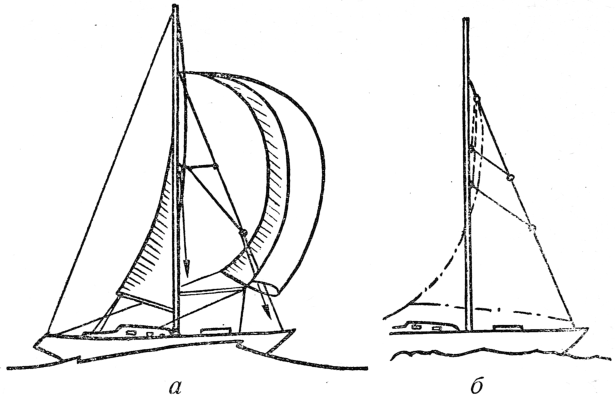
\includegraphics[scale=1.3]{0144P}
  \caption{Установка лееров против <<закручивания>> спинакера}
  \label{fig:144}
  \small
  \centering{}
  \textit{а} \--- убирание леера; \textit{б} \--- постоянные леера
\end{figure*}

\textbf{Роль прогноза в крейсерских гонках.} Для правильного и своевременного приёма метеорологических прогнозов необходимо составить таблицу с перечнем всех радиостанций (по районам), их позывных, указанием радиочастот и времени выхода в эфир. Анализируя принятые прогнозы, важно иметь в виду следующие обстоятельства: 
\begin{itemize}
\item для каждого района прогноз имеет свою вероятность оправдывания; 
\item прогноз всегда даётся обобщённый на большую площадь, а там, где находится яхта (т.\=,е. в конкретном месте), может быть другая погода; 
\item долгосрочный прогноз погоды определяет главным образом районы, откуда переносятся основные массы воздуха, например при западных ветрах для Балтийского моря \--- Северное или Норвежское море; 
\item циклоны могут перемещаться со скоростью до 500 миль в сутки, поэтому за их перемещением нужно следить по метеобюллетеням с момента зарождения. 
\end{itemize}

Своевременное получение прогнозов погоды и штормовых предупреждений, грамотный их анализ помогают приготовиться к ожидаемому ветру, наметить оптимальный маршрут гонки и выбрать наиболее целесообразную тактику на дистанции гонки.
